\documentclass[portuges,]{tufte-handout}

%\geometry{showframe}% for debugging purposes -- displays the margins

\usepackage{amsmath}

% Set up the images/graphics package
\usepackage{graphicx}
\setkeys{Gin}{width=\linewidth,totalheight=\textheight,keepaspectratio}
\graphicspath{{graphics/}}

% The following package makes prettier tables.  We're all about the bling!
\usepackage{longtable,booktabs}
% url
\usepackage{url}

% The units package provides nice, non-stacked fractions and better spacing
% for units.
\usepackage{units}

% The fancyvrb package lets us customize the formatting of verbatim
% environments.  We use a slightly smaller font.
\usepackage{fancyvrb}
\fvset{fontsize=\normalsize}

% Small sections of multiple columns
\usepackage{multicol}

% Provides paragraphs of dummy text
\usepackage{lipsum}

% These commands are used to pretty-print LaTeX commands
\newcommand{\doccmd}[1]{\texttt{\textbackslash#1}}% command name -- adds backslash automatically
\newcommand{\docopt}[1]{\ensuremath{\langle}\textrm{\textit{#1}}\ensuremath{\rangle}}% optional command argument
\newcommand{\docarg}[1]{\textrm{\textit{#1}}}% (required) command argument
\newenvironment{docspec}{\begin{quote}\noindent}{\end{quote}}% command specification environment
\newcommand{\docenv}[1]{\textsf{#1}}% environment name
\newcommand{\docpkg}[1]{\texttt{#1}}% package name
\newcommand{\doccls}[1]{\texttt{#1}}% document class name
\newcommand{\docclsopt}[1]{\texttt{#1}}% document class option name

% use symbols instead of numbers for footnotes (Caleb McDaniel)
% http://tex.stackexchange.com/questions/826/symbols-instead-of-numbers-as-footnote-markers
%\renewcommand*{\thefootnote}{\fnsymbol{footnote}}

\usepackage[portuges]{babel}

% add line numbers (Caleb McDaniel)

\title{Apostila de Biologia Evolutiva - BIO312}
%\author{ Diogo Melo - Monique Simon}
\author{\Large Diogo Melo\vspace{0.05in} \newline\normalsize Laboratório de evolução de mamíferos \(\cdot\) Universidade de São Paulo \newline\footnotesize diogro@cecm.usp.br\vspace*{0.2in}\newline \Large Monique Simon\vspace{0.05in} \newline\normalsize Laboratório de evolução de mamíferos \(\cdot\) Universidade de São Paulo \newline\footnotesize monique.nouailhetas@gmail.com\vspace*{0.2in}\newline }
%\author{Diogo Melo (Laboratório de evolução de mamíferos \(\cdot\) Universidade de São Paulo) \and Monique Simon (Laboratório de evolução de mamíferos \(\cdot\) Universidade de São Paulo)}
\date{Novembro de 2014}


\begin{document}

\maketitle




\newpage

\section{Introdução}\label{introduuxe7uxe3o}

O objetivo dessa apostila é explorar os princípios da Genética
Quantitativa, passando pelos tipos de dados tratados, sua descrição e
análise, e como isso se insere na teoria evolutiva moderna. A teoria da
Genética Quantitativa refere-se à herança de caracteres contínuos, nos
quais as diferenças entre indivíduos são quantitativas e não
qualitativas. Como exemplo, podemos pensar no caráter ``altura'' em uma
determinada população, e verificar que ele possuí uma distribuição
contínua de valores individuais, não apenas tipos distintos separados em
classes bem definidas (como textura por exemplo, lisa ou rugosa). A
compreensão da herança dos caracteres contínuos é de fundamental
importância para a teoria evolutiva, pois diferenças individuais
quantitativas constituem a base na qual a seleção natural pode atuar e
promover mudanças entre as gerações de uma população.

\section{Um pouco de história}\label{um-pouco-de-histuxf3ria}

Antes de adentrarmos nos princípios e conceitos da Genética
Quantitativa, vamos aprender um pouco sobre o contexto histórico no qual
a teoria se desenvolveu. O desabrochar da Genética Quantitativa está
intimamente relacionado com a elaboração da própria Síntese Moderna e
grandes nomes da biologia participaram nesse desenrolar da área. Os
princípios da teoria foram desenvolvidos por volta da década de 1920, em
resposta a uma histórica controvérsia na teoria evolutiva referente à
aparente incompatibilidade entre a genética mendeliana e a escola
biométrica. A primeira lidava com a herança de caracteres discretos por
meio da segregação independente dos alelos, de um ou mais loci, e o
cálculo de razões mendelianas para expressar as proporções de diferentes
genótipos da prole gerada a partir de combinações particulares de
genótipos parentais. Os mendelianos defendiam que o aparecimento de
novas macromutações (mutações de grande efeito) propiciava variação nos
caracteres discretos e sua evolução. Já a escola biométrica, liderada
por Karl Pearson e W.F.R. Weldon, focava na herança de caracteres
contínuos e na ideia de evolução como resultado da seleção natural
atuando em sua distribuição. Pearson elaborou diversos métodos para se
estudar a variação de caracteres contínuos, como as teorias de regressão
e de correlação. O grande debate entre as duas linhas de pensamento
recaia sobre a dúvida de os caracteres discretos possuírem as mesmas
propriedades de hereditariedade e evolução que os caracteres contínuos
\cite{Lynch1998}. A reconciliação foi alcançada pelos trabalhos
independentes de Ronald Fisher, J.B.S. Haldane e Sewall Wright,
culminando na elaboração da Síntese Moderna da teoria evolutiva. Fisher
(1918) demonstrou que os resultados obtidos pelos biometricistas podiam
ser derivados de princípios mendelianos, postulando a existência de
múltiplos alelos atuando sobre um único caráter (Fig. \ref{variosloci}).
Nesse artigo, ele introduz o conceito de partição de variância, que
permite a discriminação de efeitos genéticos e ambientais na
distribuição dos caracteres, extensivamente utilizado na genética
quantitativa. Os trabalhos clássicos em genética de populações de
Fisher, Haldane e Wright demonstraram que a seleção natural pode
funcionar com os tipos de variação observados em populações naturais e
com as leis de herança mendelianas. Com o debate entre mendelianos e
biometricistas resolvido, a biologia pôde ser unificada no eixo comum da
teoria evolutiva, permitindo o aprofundamento dos estudos em genética de
populações e genética quantitativa em temas macroevoutivos, como
especiação por exemplo.

\begin{figure}
  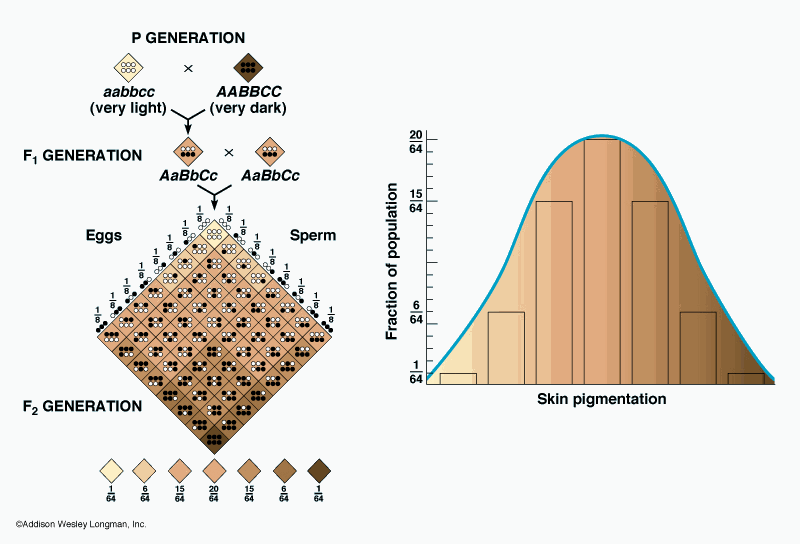
\includegraphics{./figuras/variosalelos.png}
  \caption{Vários loci podem atuar sobre o mesmo caráter, dando a
      este uma variação continua na população.}
  \label{variosloci}
  \setfloatalignment{b}
\end{figure}

\section{Princípios matemáticos em Genética
Quantitativa}\label{princuxedpios-matemuxe1ticos-em-genuxe9tica-quantitativa}

Para podermos usar a teoria da Genética Quantitativa no estudo das
propriedades genéticas e da evolução de caracteres contínuos em
populações, precisamos lançar mão de certos princípios matemáticos
relacionados com variação, como média, variância e covariância, e
relacionados com a representação destes em um morfoespaço, como vetores
e matrizes.

\section{Caracteres contínuos}\label{caracteres-contuxednuos}

Agora que temos uma noção do que são e como podem ser herdados os
caracteres contínuos, podemos pensar em quais critérios podemos utilizar
para escolher os caracteres em um estudo. É preciso garantir que as
medidas que se realizam em um indivíduo (ou em indivíduos de uma
espécie) representem os mesmos caracteres nos outros indivíduos (ou nos
indivíduos das outras espécies, no caso de estudos macroevolutivos).
Esse cuidado precisa ser tomado para que a variação que se observa nos
dados (que é o foco dos estudos quantitativos) não tenha uma fonte a
mais de erro referente a heterogeneidade de caracteres medidos entre
indivíduos ou entre espécies. O critério fundamental para garantirmos
que são os mesmos caracteres em todos os indivíduos é o de homologia.
Nós reconhecemos estruturas homólogas por serem discretas e
reconhecíveis em todos os indivíduos. Homologia implica em uma mesma
origem ancestral do caráter, e dessa maneira, podemos estudar diferenças
em caracteres homólogos em um contexto evolutivo usando de informações
de parentesco dos indivíduos amostrados.

\section{Distâncias e Vetores}\label{distuxe2ncias-e-vetores}

Uma vez escolhidos quais serão os caracteres usados no estudo,
precisamos fazer as medidas e representar esses dados de forma
conveniente. Existem diversas formas de tomar dados quantitativos: para
distâncias podemos usar paquímetros, réguas, programas de computador que
podem obter distâncias de imagens bidimensionais ou representações
tridimensionais, digitalizadores digitais; além disso, podemos tomar
medidas como peso, com uma balança; expressão gênica, quantidade de RNA
mensageiro, concentração de proteínas, atividade enzimática, todos com
técnicas de biologia molecular; pigmentação ou brilho podem ser
quantificados digitalmente. Todos esses dados representam medidas
contínuas, potencialmente herdáveis, que portanto podem ser estudadas
dentro do paradigma da genética quantitativa.

Com os dados em mão, podemos representá-los matematicamente. A maneira
mais conveniente de fazer isso é utilizando o conceito de um vetor. A
figura \ref{vetores} ilustra a representação de um par de medidas
utilizando um vetor bidimensional. A partir dessa abstração, podemos
construir uma teoria bastante completa.

\begin{marginfigure}
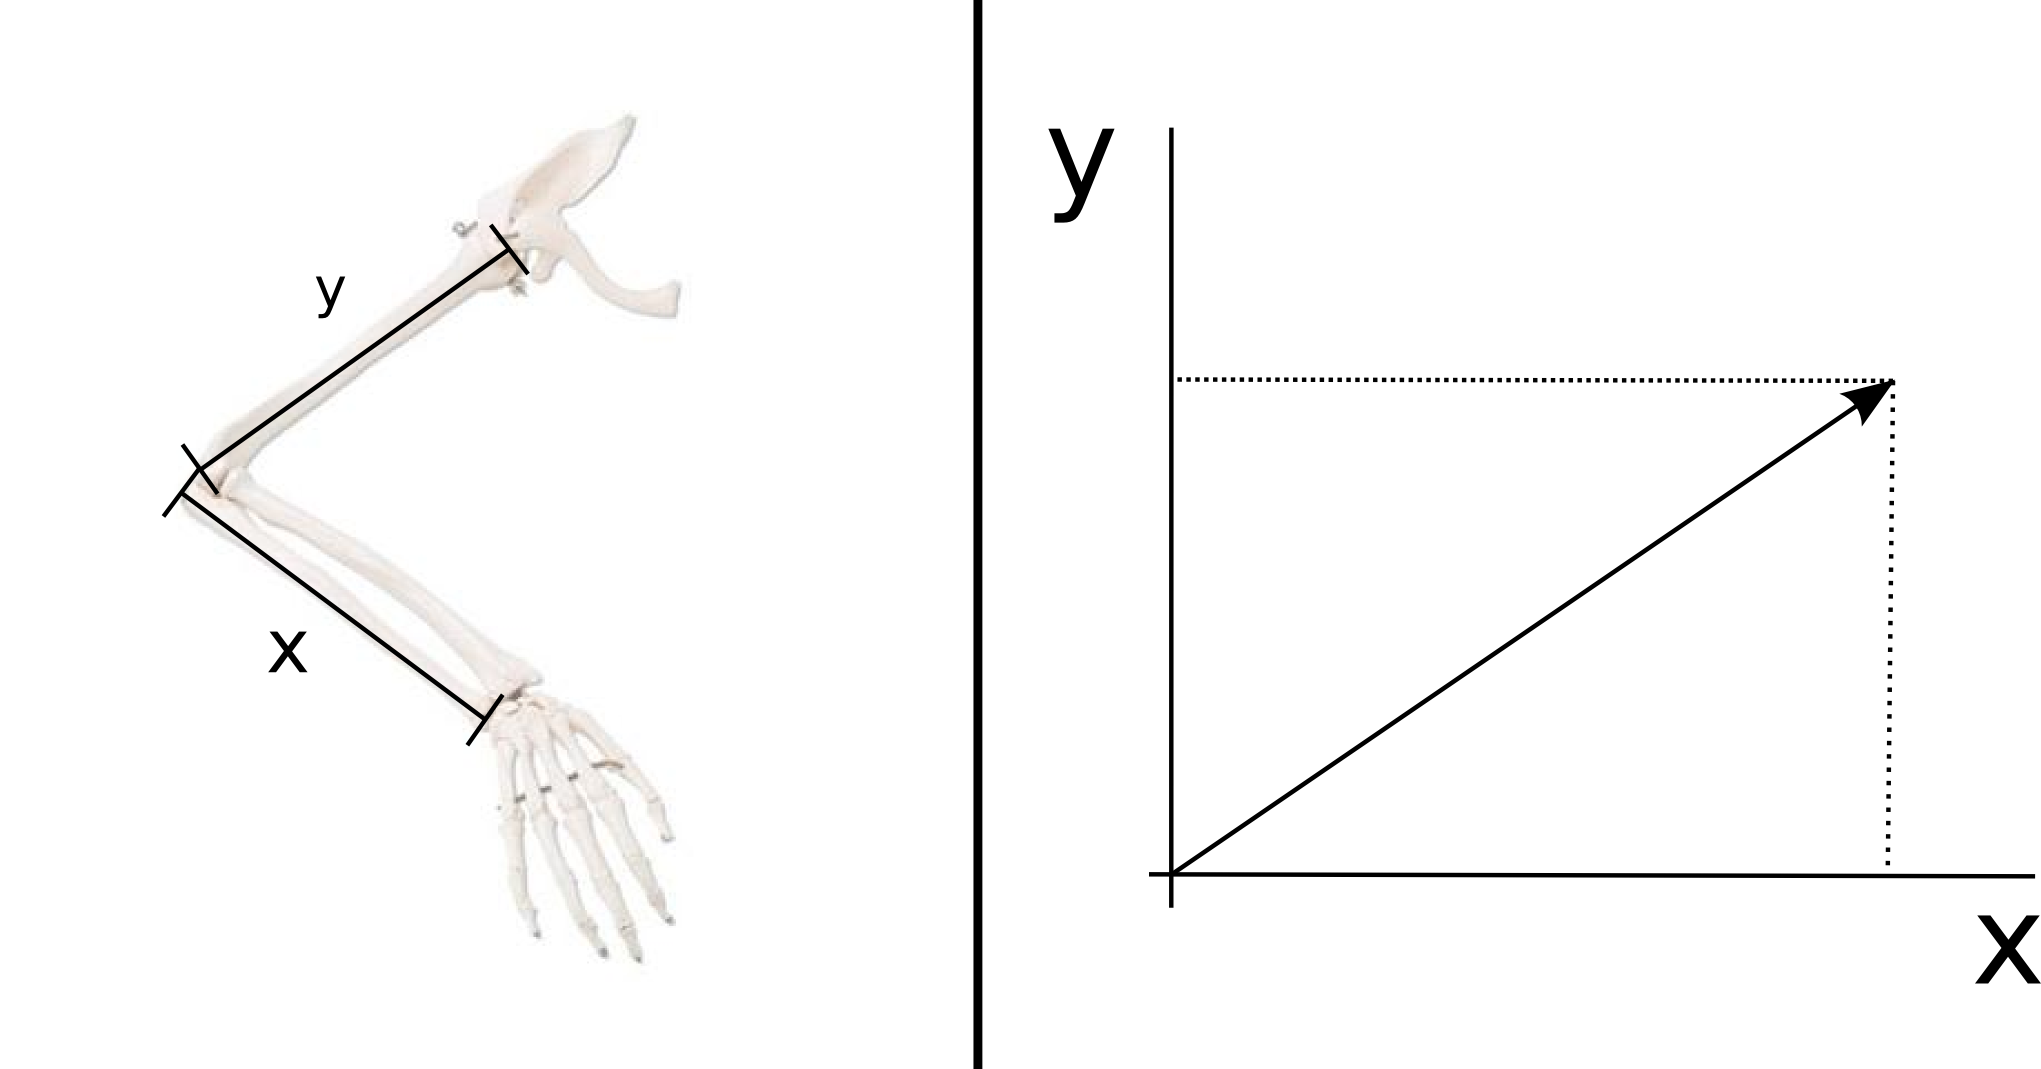
\includegraphics{./figuras/medidas-vetores.png}
\caption{Representação de medidas reais na forma vetorial.
Vemos duas medidas de tamanho linear de ossos do braço representadas num
vetor.}
\label{vetores}
\end{marginfigure}

No plano \((x,y)\) representado na figura \ref{vetores}, podemos
representar qualquer combinação de tamanhos do braço e do antebraço. Por
exemplo, na convenção da figura \ref{vetores}, um individuo com 15 cm de
braço e 20 cm de antebraço é representando pelo vetor \((20, 15)\).
Qualquer fenótipo do tamanho desses dois ossos pode ser descrito por um
par de números. Como todos os fenótipos possíveis estão representados
nesse plano, ele é chamado de morfoespaço.

No morfoespaço bidimensional, ou mesmo tridimensional, os vetores
representando os fenótipos podem ser visualizados com facilidade. Porém,
em genética quantitativa, é comum trabalharmos com um número muito maior
de medidas, chegando até centenas variáveis observadas em cada
indivíduo. Ainda assim, podemos continuar representando nossos
indivíduos por vetores, agora compostos por muito mais números,
representando todas as medidas tomadas. Para 4 medidas, por exemplo, os
vetores são listas de 4 números, como \((4.94, 9.94, 15.11, 20.17)\),
cada um representando um dado caráter de um indivíduo. O morfoespaço
nesse caso seria um hiperplano com 4 dimensões.

\begin{marginfigure}
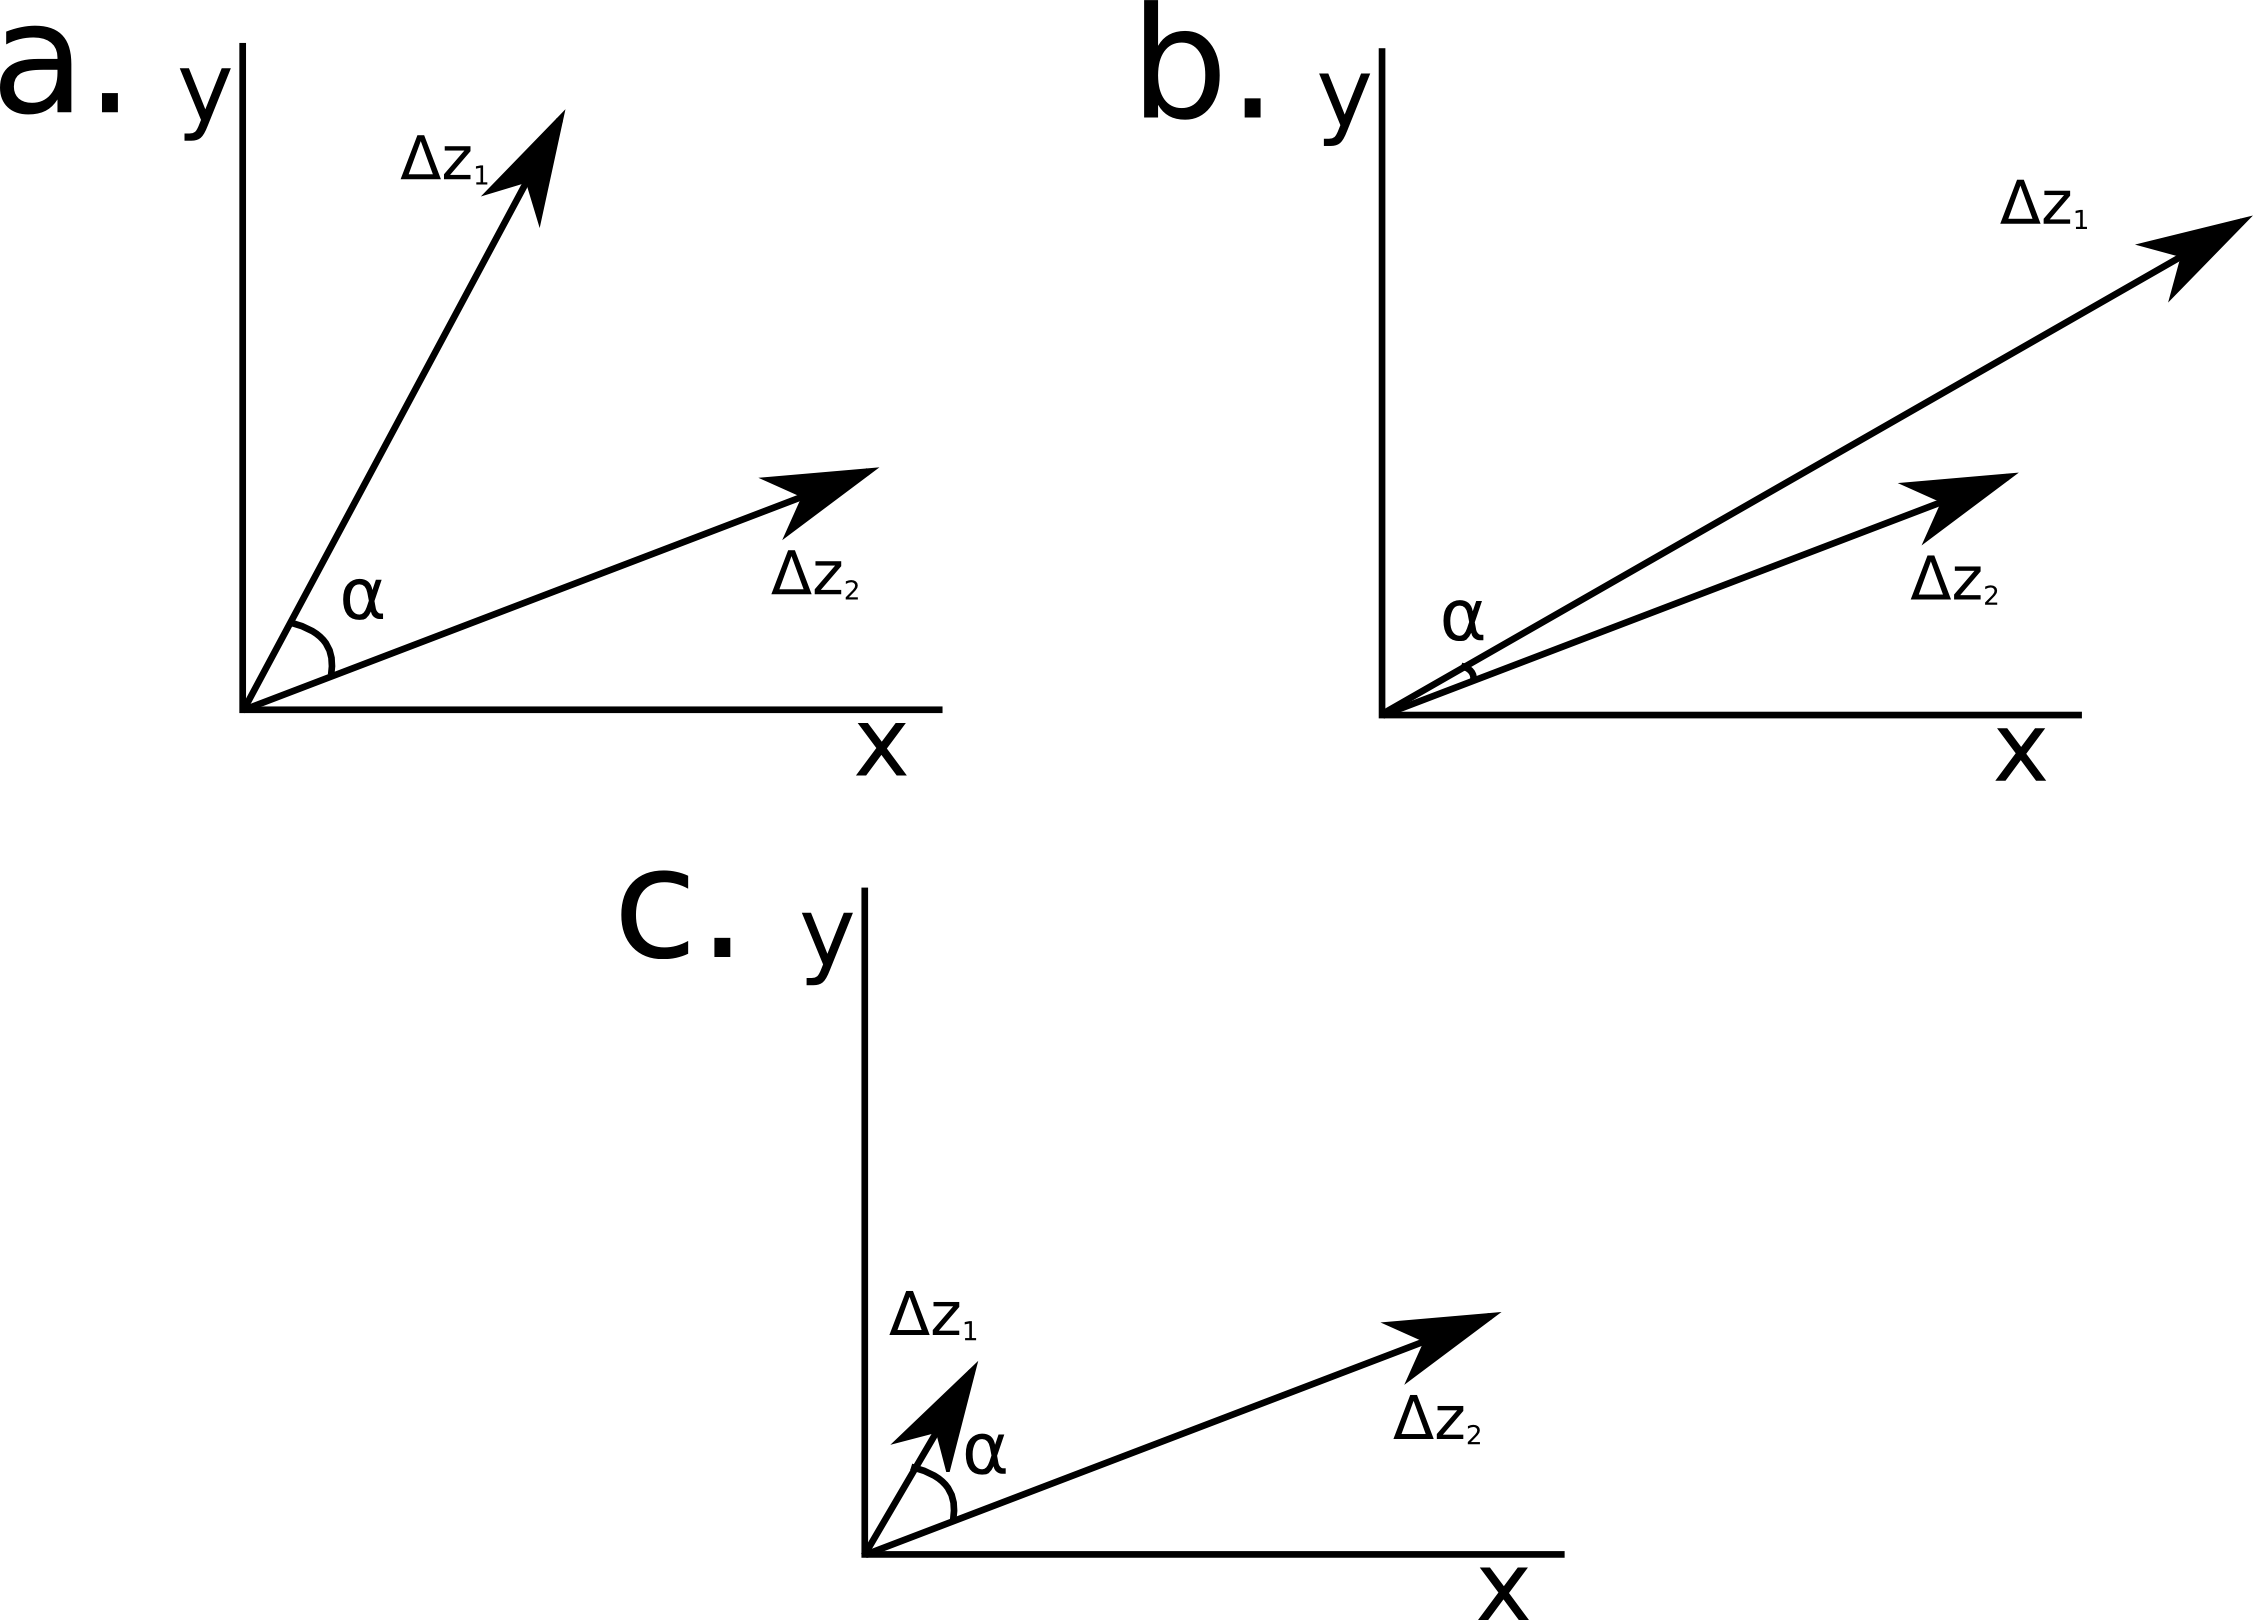
\includegraphics{./figuras/deltazes.png}
\caption{Possíveis mudanças nas médias de duas populações. No
caso (a) magnitudes de mudança iguais mas direções diferentes. (b)
direções iguais mas magnitudes diferentes e (c) magnitudes e direções
diferentes.}
\label{deltazes}
\end{marginfigure}

Vetores podem representar também mudanças em fenótipos. Suponha que a
média bivariada de uma população tenha se alterado entre os momentos a e
b, passando de \(\overline z_a=(10, 50)\) para
\(\overline z_b=(15, 47)\). Essa mudança pode ter uma série de motivos,
um episodio de seleção direcional ou um gargalo populacional, por
exemplo. Podemos representar essa mudança na média como um vetor:

\[
\overline z_b - \overline z_a = \Delta \overline z_{ba} = (15, 47)_b - (10, 50)_a = (5, -3)
\]

Ou seja, o primeiro caráter aumentou em 5 unidades na sua média,
enquanto o segundo caráter diminuiu em 3 unidades. O vetor de mudança,
\(\Delta \overline z\), representa matematicamente o evento evolutivo.

\section{Comparação de Vetores}\label{comparauxe7uxe3o-de-vetores}

Frequentemente estaremos interessados em comparar vetores. Por exemplo,
será que as mudanças nas médias de duas populações foram na mesma
direção do morfoespaço? Caso não tenham sido, quão diferentes são elas?
Nas próximas seções, veremos casos onde essas perguntas aparecem de
forma bastante natural em outros contextos. Para isso, precisamos de uma
forma de comparar vetores, tanto em suas magnitude quando em suas
direção. A figura \ref{deltazes} mostra algumas possibilidades para as
diferenças entre vetores de mudanças evolutivas de duas populações.

Vemos, então, que uma forma natural de comparar vetores é
representando-os pela sua magnitude e direção.

\section{Magnitude ou norma de
vetores}\label{magnitude-ou-norma-de-vetores}

Para calcular a magnitude de um vetor, podemos nos valer da teorema de
Pitágoras para triângulos retângulos (figura \ref{pitagoras}). Para um
vetor \(\Delta z\) com componentes \((\Delta z_x, \Delta z_y)\), podemos
calcular sua norma (ou magnitude) \(|\Delta z|\) como:

\[
|\Delta z| = \sqrt{\Delta z_x^2 + \Delta z_y^2}
\]

A boa notícia é que essa formula continua valendo para dimensionalidades
altas. Suponha que queiramos calcular a norma de um vetor em 4 dimensões
\(\Delta z = (\Delta z_x, \Delta z_y, \Delta z_z, \Delta z_w)\). A conta
seria simplesmente:

\[
|\Delta z| = \sqrt{\Delta z_x^2 + \Delta z_y^2+ \Delta z_z^2 + \Delta z_w^2}
\]

Para um vetor de dimensionalidade arbitraria
\(\mathbf{x} = (x_1, x_2, \cdots, x_p)\), sua norma pode ser expressa
como:

\[
|\mathbf{x}| = \sqrt{\sum_{i=1}^p x_i^2}
\]

\begin{marginfigure}
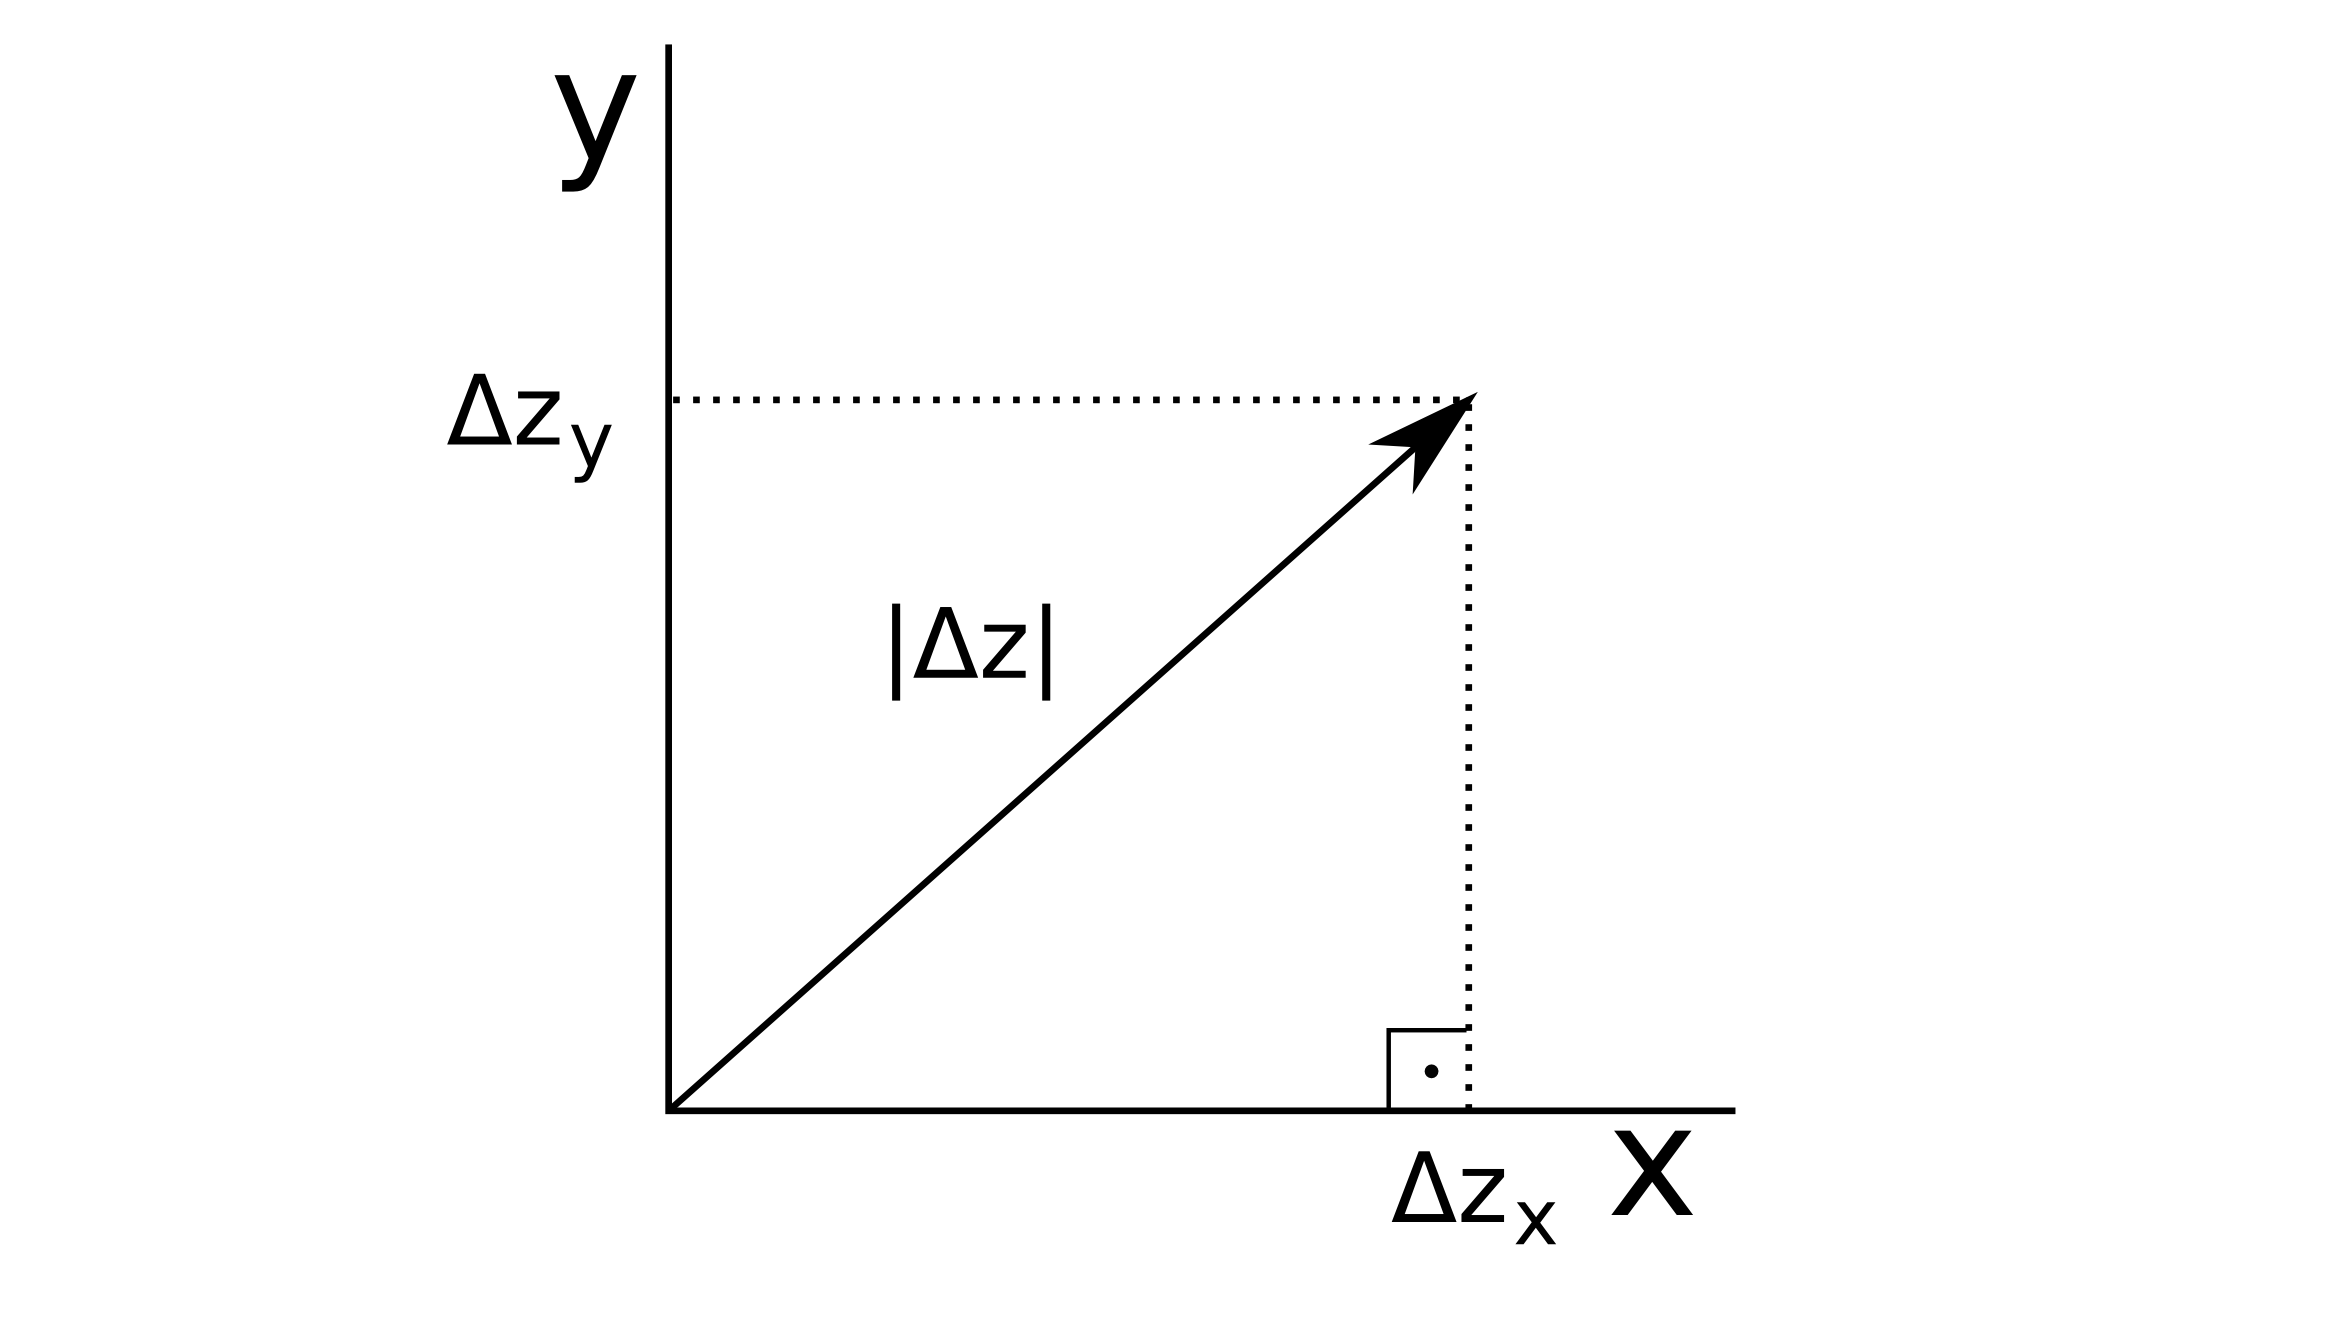
\includegraphics{./figuras/pitagoras.png}
\caption{Calculando a norma ou magnitude de um vetor pelo
Teorema de Pitágoras.}
\label{pitagoras}
\end{marginfigure}

\section{Correlação de vetores}\label{correlauxe7uxe3o-de-vetores}

Além de comparações de magnitudes, podemos comparar vetores pelo angulo
formado entre eles, ou seja, a diferença em suas direções. Uma escala
bastante conveniente é a do cosseno do angulo formado entre dois
vetores. Caso eles tenham a mesma direção, o cosseno do angulo entre
eles é um, caso eles tenham direções completamente ortogonais, ou seja,
um angulo de 90 graus entre deles, o cosseno do angulo é zero. Caso os
vetores apontem para direções opostas, formando um angulo de 180 graus,
o cosseno do angulo entre eles é -1. O cosseno do angulo entre dois
vetores também é chamado de correlação de vetores. Para calcular o
cosseno do angulo entre dois vetores a partir de suas componentes,
devemos fazer uso da lei dos cossenos (figura \ref{leidoscossenos}).
Utilizando a notação da figura \ref{leidoscossenos}, a correlação entre
os vetores \(\Delta z_1 = (\Delta z_{11}, \Delta z_{12})\) e
\(\Delta z_2 = (\Delta z_{21}, \Delta z_{22})\) seria:

\[
Corr(\Delta z_1, \Delta z_2) = cos(\alpha) = \frac{(\Delta z_{11}  \Delta z_{21}) + (\Delta z_{12}  \Delta z_{22})}{| \Delta z_1|  | \Delta z_2|} = \frac{(\Delta z_{11}  \Delta z_{21}) + (\Delta z_{12}  \Delta z_{22})}{\sqrt{\Delta z_{11}^2 + \Delta z_{12}^2}  \sqrt{\Delta z_{21}^2 + \Delta z_{22}^2}}
\]

Em outras palavras, o cosseno do angulo \(\alpha\) é calculado como a
soma dos produtos cruzados entre os dois vetores dividido pela sua
norma. O termo de soma dos produto cruzados,
\((\Delta z_{11} \Delta z_{21}) + (\Delta z_{12} \Delta z_{22})\), é
conhecido como o produto escalar entre dos vetores, e pode ser
generalizado para um numero arbitrário de dimensões. Para dois vetores
\(\mathbf{x} = (x_1, x_2, \cdots, x_p)\) e
\(\mathbf{y} = (y_1, y_2, \cdots, y_p)\), o seu produto escalar é
definido como:

\[
\mathbf{x} \cdot \mathbf{y} = \sum_{i=1}^p x_iy_i
\]

Com isso, podemos definir a correlação de vetores de qualquer dimensão
como:

\[
Corr(\mathbf{x}, \mathbf{y}) = \frac{\mathbf{x} \cdot \mathbf{y}}{|\mathbf{x}||\mathbf{y}|}
\]

\begin{marginfigure}
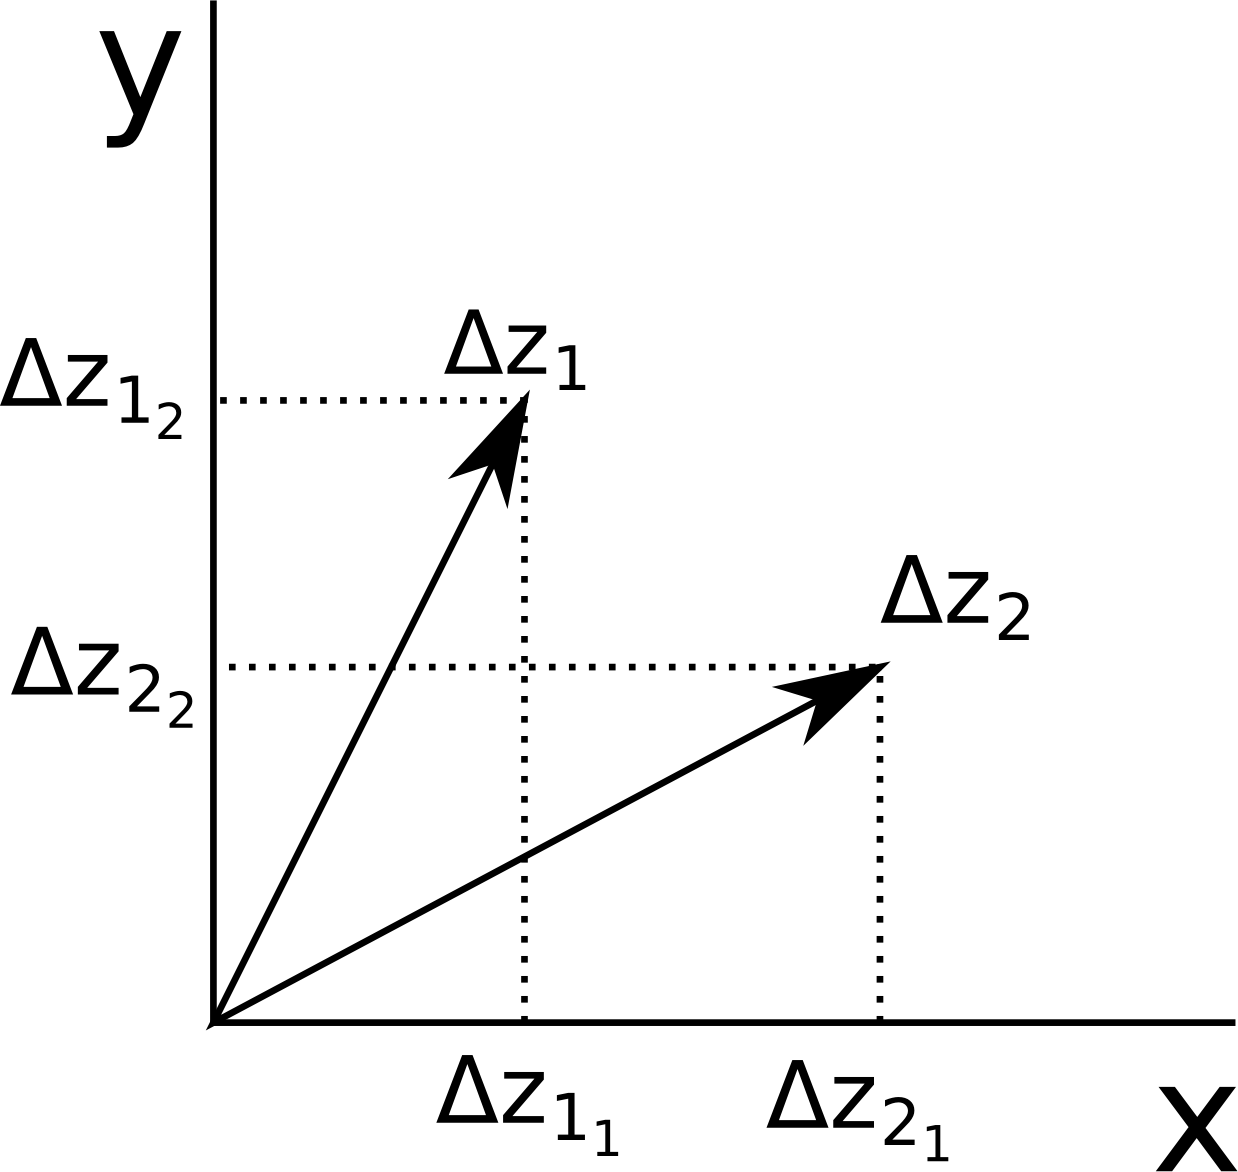
\includegraphics{./figuras/leidoscossenos.png}
\caption{Utilizando a lei dos cossenos para calcular o cosseno
do angulo \(\alpha\) entre dois vetores.}
\label{leidoscossenos}
\end{marginfigure}

\section{Normalização de vetores}\label{normalizauxe7uxe3o-de-vetores}

Para populações uma mesma espécie, onde os indivíduos são relativamente
parecidos, a magnitude de um vetor de mudança evolutiva traz informações
importantes quando comparamos populações nas suas mudanças evolutivas.
No entanto, se vamos trabalhar com espécies de tamanhos e níveis de
variações muito diferentes, comparar a magnitude da resposta passa a ser
pouca informativa. Esse efeito é claro quando pensamos, por exemplo, na
escala geral das diferentes espécies. Um variação de 1cm no tamanho
médio do antebraço de uma população de cavalos pode ser insignificante,
mas uma mudança de mesmo tamanho em uma população de camundongos é
brutal. Portanto, comparar a norma da resposta evolutiva entre
populações com escalas diferentes é uma métrica que não faz sentido
biológico. Quando estamos interessados somente na direção dos vetores
estudados, é conveniente, então, padronizar a magnitude dos vetores de
todas as populações ou espécies envolvidas na analise. Normalmente
modificamos os vetores para que eles tenham magnitude unitária, ou seja,
igual a 1. Esse procedimento é chamado de normalização, e se
\(\mathbf{x_N}\) é normalizado, então \(|\mathbf{x_N}| = 1\).

Suponha que \(\mathbf{x}\) seja um vetor não normalizado (então
\(|\mathbf{x}| \neq 1\)), como fazemos para obter sua versão normalizada
\(\mathbf{x_N}\)? Basta dividir todos os elementos de \(\mathbf{x}\) por
\(|\mathbf{x}|\)! Note que:

\[
|\mathbf{x}| = \sqrt{\sum_{i=1}^p x_i^2}
\]

Então:

\[
|\mathbf{x_N}| = \left| \frac{\mathbf{x}}{|\mathbf{x}|} \right| = \sqrt{\sum_{i=1}^p \left (\frac{x_i}{|\mathbf{x}|} \right )^2} = \frac{1}{|\mathbf{x}|} \sqrt{\sum_{i=1}^p x_i^2} = \frac{|\mathbf{x}|}{|\mathbf{x}|} = 1
\]

Outra vantagem de usar vetores normalizados é na hora do calculo de suas
correlações. Se \(\mathbf{x}\) e \(\mathbf{y}\) são normalizados, sua
correlação é simplesmente seu produto interno (ou a soma dos seus
produtos cruzados), pois:

\[
Corr(\mathbf{x}, \mathbf{y}) = \frac{ \mathbf{x} \cdot \mathbf{y} }{|\mathbf{x}||\mathbf{y}|} = \frac{ \mathbf{x} \cdot \mathbf{y} }{1 \cdot 1} =  \mathbf{x} \cdot \mathbf{y} = \sum_{i=1}^p x_iy_i
\]

\section{Variâncias, Covariâncias e
Correlações}\label{variuxe2ncias-covariuxe2ncias-e-correlauxe7uxf5es}

\section{Um caráter}\label{um-caruxe1ter}

O estudo dos caracteres contínuos é centrado em sua variação, uma vez
que é em termos de variação que as questões genéticas primárias são
formuladas. A quantidade de variação é medida e expressa como a
variância. A variância é uma medida comum, que quantifica desvios de
cada indivíduo em relação à média global. A variância de um caráter
contínuo \(z\), expresso em uma população com \(n\) indivíduos \(z_1\) a
\(z_n\), e média \(\overline z\), é dada por:

\[
var(z) = \frac{1}{n-1}\sum_{i=1}^n (z_i - \overline z)^2
\]

O procedimento para calculo da variância é, então, bastante simples:
basta calcular a diferença de cada indivíduo da média, elevar essas
diferenças ao quadrado, somar todas e dividir pelo número de indivíduos
menos um.

Como as diferenças da média são elevadas ao quadrado, a variância tem
unidades quadráticas em relação às unidades iniciais. Ou seja, se
estamos trabalhando com distâncias, e medindo os caracteres em cm, a
variância tem unidades de cm\(^2\). Alternativamente, podemos trabalhar
com a raiz quadrada da variância, chamada desvio padrão, que tem
unidades iguais às medidas originais e frequentemente é mais simples de
ser interpretada intuitivamente. Em uma distribuição normal, 95\% dos
indivíduos se encontra a uma distância de, no máximo, 2 desvios padrões
da média. Ainda outra possibilidade, caso queiramos comparar populações
com escalas muito distintas, é medir variação em uma escala
adimensional. Um exemplo de estatística adimensional de variação é o
coeficiente de variação, que nada mais é que a razão entre o desvio
padrão e a média da população. Para caracteres ósseos de mamíferos,
esperamos um coeficiente de variação por volta de 0.1, ou seja, o desvio
padrão é cerca de 10\% dá média. Essas regras gerais podem ser bastante
úteis quando confrontados com dados pela primeira vez, pois permitem
rapidamente identificar particularidades ou erros nas medidas.

\section{Mais de um caráter}\label{mais-de-um-caruxe1ter}

Quando trabalhamos com mais de um caráter, além de quantificar a
variância individual de cada um, devemos também medir a interação entre
eles. Esse tipo de medida é fundamental no estudo de modularidade, como
veremos nas próximas seções.

De forma análoga ao calculo da variância, a covariância mede a variação
conjunta de dois caracteres. Para dois caráteres \(z_1\) e \(z_2\),
expressos em uma população com \(n\) indivíduos, com médias
\(\overline z_1\) e \(\overline z_2\), a covariância entre eles é dada
por:

\[
cov(z_1, z_2) = \frac{1}{n-1} \sum_{i=1}^n (z_{1i} - \overline z_1)(z_{2i} - \overline z_2)
\]

Ou seja, a média do produto entre as diferenças da média para os
caracteres de cada indivíduo.

Se os desvios da média dos dois caracteres forem na mesma direção, ou
seja, se um crescer ou diminuir junto com o outro em cada indivíduo, a
covariação será alta. Ou, se os desvios forem em direções opostas, com
um aumentando e o outro diminuindo, a covariação será negativa. Se,
ainda, os desvios não tiverem relação nenhuma, desvios coordenados e
opostos tendem a se cancelar, e a covariação será próxima de zero.

Suponha agora que estivéssemos estudando um grande número de caracteres
métricos, numerados de \(1\) a \(p\), que descrevem de forma completa
alguma estrutura anatômica. O fenótipo de cada um dos \(n\) indivíduos
da população estudada pode ser representado por um vetor
\(\mathbf{z}_j = (z_{1j}, z_{2j}, \cdots, z_{pj})\). Como podemos
descrever a variação nessa população? Primeiro, calculamos o vetor de
médias da população,
\(\mathbf{\overline z} = (\overline z_1, \overline z_2, \cdots, \overline z_p)\),
onde:

\[
\overline z_i = \frac{1}{n} \sum_{j=1}^n z_{ij}
\]

Lembre-se que \(z_{ij}\) significa o caráter \(i\) do indivíduo \(j\).

Com as médias, podemos calcular a variância de cada caráter na
população:

\[
var(z_i) = \frac{1}{n-1} \sum_{j=1}^n (z_{ij} - \overline z_i)^2
\]

E, como são muitos caracteres, devemos também calcular a covariâncias
entre eles:

\[
cov(z_i, z_k)_{i \ne k} = \frac{1}{n-1} \sum_{j=1}^n (z_{ij} - \overline z_i)(z_{kj} - \overline z_k)
\]

Vale notar que a fórmula da covariância se torna igual a da variância
quando \(i=k\).

\section{Correlação}\label{correlauxe7uxe3o}

Assim como no caso da variância, a covariância sofre efeitos da escala
da medida em questão. Caracteres maiores tendem a ter covariâncias mais
altas que caracteres menores. Para contornar esse problema, podemos
escalonar as covariâncias pelas variâncias, dividindo a covariância pela
raiz do produto das variâncias.

\[
Corr(x, y) = \frac{cov(x, y)}{\sqrt(var(x)var(y))} = \frac{\sum_{i=1}^n (x_i - \overline x)(y_i - \overline y)}{(\sum_{j=1}^n (x_j - \overline x)^2\sum_{j=1}^n(y_j - \overline y)^2)^{1/2}}
\]

Como ambas as quantidades são representadas em unidades quadráticas, a
estatística resultante, chamada correlação, é adimensional e varia de -1
a 1. Correlação zero indica que as variáveis não tem relação linear,
enquanto correlação de 1 ou -1 indica total dependência entre as
variáveis, variando da mesma direção no caso de correlação positiva, e
variando em sentido oposto no caso de correlação negativa. Por ser
adimensional e sempre variar entre -1 e 1, a correlação pode ser
comparada entre pares de caracteres ou entre populações diferentes.

Vale ressaltar que, caso as médias das variáveis sejam zero, a formula
apresentada para correlação entre medidas se reduz à formula de
correlação ou cosseno entre vetores, justificando o uso do mesmo nome
para a correlação entre medidas e a correlação de vetores.

\section{Matrizes}\label{matrizes}

Variâncias, covariâncias e correlações são formas de descrever a
variação de caracteres morfológicos, e, frequentemente, estudamos um
grande número de caracteres descrevendo uma estrutura complexa. Como
podemos organizar todas essas estatísticas de forma a representar a
variação de uma estrutura formada de vários caracteres? A representação
matricial resolve esse problema, além de fornecer muitas facilidades
matemáticas e computacionais no estudo da variação em populações
biológicas.

Suponha que estejamos trabalhando com dois caráteres, \(x\) e \(y\),
medidos em uma população qualquer que descrevem uma estrutura \(z\).
Após a medição, calculamos as médias, \(\overline x\) e \(\overline y\),
as variâncias, \(var(x)\) e \(var(y)\), e, por fim, as covariâncias e
correlações \(cov(x, y)\) e \(corr(x, y)\). Como esses dados seriam
representados? As médias seriam um vetor
\(\overline z = (\overline x, \overline y)\). Já as variâncias e
covariâncias seriam organizadas em uma matriz, chamada matriz de
variância-covariância, ou, simplesmente, matriz de covariância. A
estrutura dessa matriz seria:

\[
Var(z) = \left (
\begin{smallmatrix}
var(x) & cov(x, y) \\
cov(x,y) & var(y)  \\
\end{smallmatrix}
\right )
\]

Ou seja, na diagonal, temos as variâncias de cada medida, e, fora da
diagonal, as covariâncias. A matriz de correlação tem exatamente a mesma
forma, porem com \(1\) na diagonal, representando a correlação de uma
medida com ela mesma.

\[
Corr(z) = \left (
\begin{smallmatrix}
1 & corr(x, y) \\
corr(x,y) & 1  \\
\end{smallmatrix}
\right )
\]

Essas representações de estendem trivialmente para dimensões mais altas.
Por exemplo, se medirmos \(p\) distâncias de uma estrutura
\(z = (z_1, z_2, \cdots, z_n)\), sua matriz de covariância seria:

\[
Var(z) = \left (
\begin{matrix}
var(z_1) & cov(z_1, z_2) & \cdots & cov(z_1, z_p) \\
cov(z_1, z_2) & var(z_2) & \cdots & cov(z_2, z_p) \\
\vdots & \vdots  & \ddots & \vdots                \\
cov(z_1, z_p) & cov(z_1, z_p) & \cdots & var(z_p) \\
\end{matrix}
\right )
\]

\section{Operações com Matrizes}\label{operauxe7uxf5es-com-matrizes}

Para trabalhar com matrizes, precisamos relembrar algumas regras de
operação matricial. A mais simples é a soma de matrizes, que é feita
simplesmente somando os elementos equivalentes. Para somar matrizes duas
matrizes \(\mathbf{A}\) e \(\mathbf{B}\), elas devem ter a mesma
dimensão. Por exemplo, se \(\mathbf{A}\) e \(\mathbf{B}\) forem matrizes
\(2\) por \(2\):

\[
\mathbf{A} + \mathbf{B} =
\left (
\begin{matrix}
A_{11} & A_{12}\\
A_{21} & A_{22}  \\
\end{matrix}
\right )
+
\left (
\begin{matrix}
B_{11} & B_{12}\\
B_{21} & B_{22}  \\
\end{matrix}
\right )
=
 \left (
\begin{matrix}
A_{11}+B_{11} & A_{12}+B_{12}\\
A_{21}+B_{21} & A_{22}+B_{22} \\
\end{matrix}
\right )
\]

Outra operação comum é a de multiplicação de matrizes. Essa operação já
é mais complicada, e NÃO se resume apenas a multiplicar os elementos
equivalentes. Na multiplicação de matrizes, uma dada posição é definida
como o produto escalar entre a linha equivalente da primeira matriz com
a coluna da segunda. Ou seja, a posição \(ij\) da matriz produto é o
poduto escalar da linha \(i\) da primeira matriz com a coluna \(j\) da
segunda. Isso significa que, em geral, \(\mathbf{A}\mathbf{B}\) pode ser
diferente de \(\mathbf{B}\mathbf{A}\). Para que essa operação seja
possivel, a primeira matriz deve ter o mesmo numero que linhas que a
segunda tenha de colunas. A matriz desultante terá o mesmo numero de
linhas que a primeira e o mesmo numero de colunas que a segunda. Se
\(\mathbf{A}\) for uma matriz \(3\) por \(2\) e \(\mathbf{B}\) uma
matriz \(2\) por \(3\), o produto entre elas seria a seguinte matrix
\(3\) por \(3\):

\[
\mathbf{A}\mathbf{B} =
\left (
\begin{matrix}
A_{11} & A_{12} \\
A_{21} & A_{22}  \\
A_{31} & A_{32} \\
\end{matrix}
\right )
\left (
\begin{matrix}
B_{11} & B_{12} & B_{13} \\
B_{21} & B_{22} & B_{23} \\
\end{matrix}
\right )
=
\left (
\begin{smallmatrix}
A_{11}B_{11} +  A_{12}B_{21} & A_{11}B_{12} +  A_{12}B_{22} & A_{11}B_{13} +  A_{12}B_{23} \\
A_{21}B_{11} +  A_{22}B_{21} & A_{21}B_{12} +  A_{22}B_{22} & A_{21}B_{13} +  A_{22}B_{23} \\
A_{31}B_{11} +  A_{32}B_{21} & A_{31}B_{12} +  A_{32}B_{22} & A_{31}B_{13} +  A_{32}B_{23} \\
\end{smallmatrix}
\right )
\]

Na verdade, o caso mais interessante para nós será o de multiplicação de
uma matriz por um vetor, que pode ser pensado como uma matriz de uma
coluna. A mesma regra vale, e temos, para uma matriz \(\mathbf{A}\) e um
vetor \(\mathbf{x}\):

\[
\mathbf{A}\mathbf{x}  =
\left (
\begin{matrix}
A_{11} & A_{12} & A_{13}\\
A_{21} & A_{22} & A_{23} \\
A_{31} & A_{32} & A_{33}\\
\end{matrix}
\right )
\left (
\begin{matrix}
x_{1}  \\
x_{2}   \\
x_{3}  \\
\end{matrix}
\right )
=
\left (
\begin{matrix}
A_{11}x_{1} +  A_{12}x_{2} +  A_{13}x_{3}\\
A_{21}x_{1} +  A_{22}x_{2} +  A_{23}x_{3}\\
A_{31}x_{1} +  A_{32}x_{2} +  A_{33}x_{3}\\
\end{matrix}
\right )
\]

Uma última operação importante, que geralmente é feita de forma
exclusivamente computacional, devido à sua dificuldade operacional, é a
de inversão de matrizes. A inversão permite definir o análogo matricial
de divisão. A inversa de uma matriz \(\mathbf{A}\) é denominada
\(\mathbf{A}^{-1}\) e definida pela propriedade:

\[
\mathbf{A}\mathbf{A}^{-1} = \mathbf{A}^{-1}\mathbf{A} = \mathbf{I}
\]

onde \(\mathbf{I}\) representa a matriz identidade, que tem apenas 1 na
diagonal e zero fora dela. A matriz identidade é o elemento neutro da
multiplicação de matrizes, ou seja:

\[
\mathbf{A}\mathbf{I} = \mathbf{I}\mathbf{A} = \mathbf{A}
\]

Isso é exatamente análogo à divisão nos numero reais, por exemplo:

\[
aa^{-1} = a^{-1}a = a\frac{1}{a} = 1
\]

como exercício, verifique que as seguintes matrizes são inversa uma da
outra:

\[
\left (
\begin{matrix}
1 & 2 \\
2 & 1 \\
\end{matrix}
\right )
\text{ e }
\left (
\begin{matrix}
-1/3 & 2/3 \\
2/3 & -1/3 \\
\end{matrix}
\right )
\]

\section{Comparação de Matrizes}\label{comparauxe7uxe3o-de-matrizes}

Nas próximas seções, vamos abordar como a estrutura de covariação das
populações pode alterar suas propriedade evolutivas. Como os padrões de
covariação variam entre populações, precisamos de técnicas para comparar
padrões de populações e especies diferentes que tragam informações sobre
as propriedades evolutivas das mesmas.

Para matrizes de covariância, podemos usar a técnica de \emph{Random
Skewers} \cite{Cheverud2007}, baseada na equação de resposta à
seleção de Lande, que veremos em detalhes nas próximas seções.
Operacionalmente, essa técnica é baseada em multiplicar duas matrizes a
serem comparadas pelo mesmo vetor de seleção e calcular a correlação
entre os vetores resultantes. Repetindo esse procedimento para milhares
de vetores de entrada, temos um estatistica que mede a semelhança de
duas matrizes num contexto evolutivo. Para duas matrizes \(\mathbf{A}\)
e \(\mathbf{B}\), a correlação de \emph{Random Skewers} é definida como:

\[
RS(\mathbf{A}, \mathbf{B}) = E[Corr(Ax, Bx)]_x
\]

onde \(E[\cdot]_x\) representa o valor esperado, ou média, para todos os
valores de vetores aleatórios \(x\).

Já para as matrizes de correlação, podemos tratar cada entrada da matriz
como uma observação e simplemente correlacionar os valores entre as duas
matrizes.

\section{Propriedades genéticas de
populações}\label{propriedades-genuxe9ticas-de-populauxe7uxf5es}

Antes de usarmos os princípios matemáticos acima descritos para
estudarmos a herança e evolução dos caracteres contínuos em populações,
vamos olhar as propriedades genéticas dos caracteres nas populações.
Para tanto, precisamos conseguir fazer a conexão entre frequência de
genes e genótipos com as diferenças quantitativas observadas em
caracteres contínuos. Essa conexão é feita com a compreensão dos
conceitos de valores genotípico e fenotípico, efeito médio de um alelo,
valor de acasalamento e partição de variância. Nas seções seguintes
veremos as definições desses conceitos. O texto a seguir foi adaptado de
Falconer e Mackay \cite{Falconer1996}.

\section{Valores genotípico e
fenotípico}\label{valores-genotuxedpico-e-fenotuxedpico}

O valor observado para um caráter medido em um indivíduo qualquer é o
valor fenotípico desse indivíduo. Para podermos analisar as propriedades
genéticas de populações, temos que dividir o valor fenotípico em
componentes atribuídos a diferentes causas: influência do genótipo e
influência do ambiente (considerando todas as circunstâncias
não-genéticas que influenciam o fenótipo). Podemos pensar que o genótipo
confere um determinado valor de um caráter ao indivíduo, e o ambiente
causa um desvio desse valor (ao fazer isso, estamos ignorando interações
genótipo-ambiente):

\[
P = G + E,
\]

sendo P o valor fenotípico, G o valor genotípico e E o desvio ambiental.
Assume-se que o desvio ambiental médio em uma população é zero, pois
consideramos que os desvios individuais ocorrerem em diversas direções
de forma independente do genótipo, e, na média, se cancelam. Assim, o
valor médio fenotípico é equivalente ao valor médio genotípico em uma
população. Essa suposição é fundamental, pois permite que estudemos as
propriedades genéticas das populações por meio de seus fenótipos, que é,
na prática, o que pode ser mensurado nos indivíduos.

Para definir os conceitos de efeito médio de um alelo e valor de
acasalamento, podemos utilizar valores arbitrários para os genótipos de
um único locus com dois alelos, \(A_1\) e \(A_2\), sendo +a, valor
genotípico do homozigoto \(A_1\)\(A_1\); -a, valor do homozigoto
\(A_2\)\(A_2\); e finalmente d, valor do heterozigoto \(A_1\)\(A_2\)
(Fig. \ref{valgen}).

\begin{marginfigure}
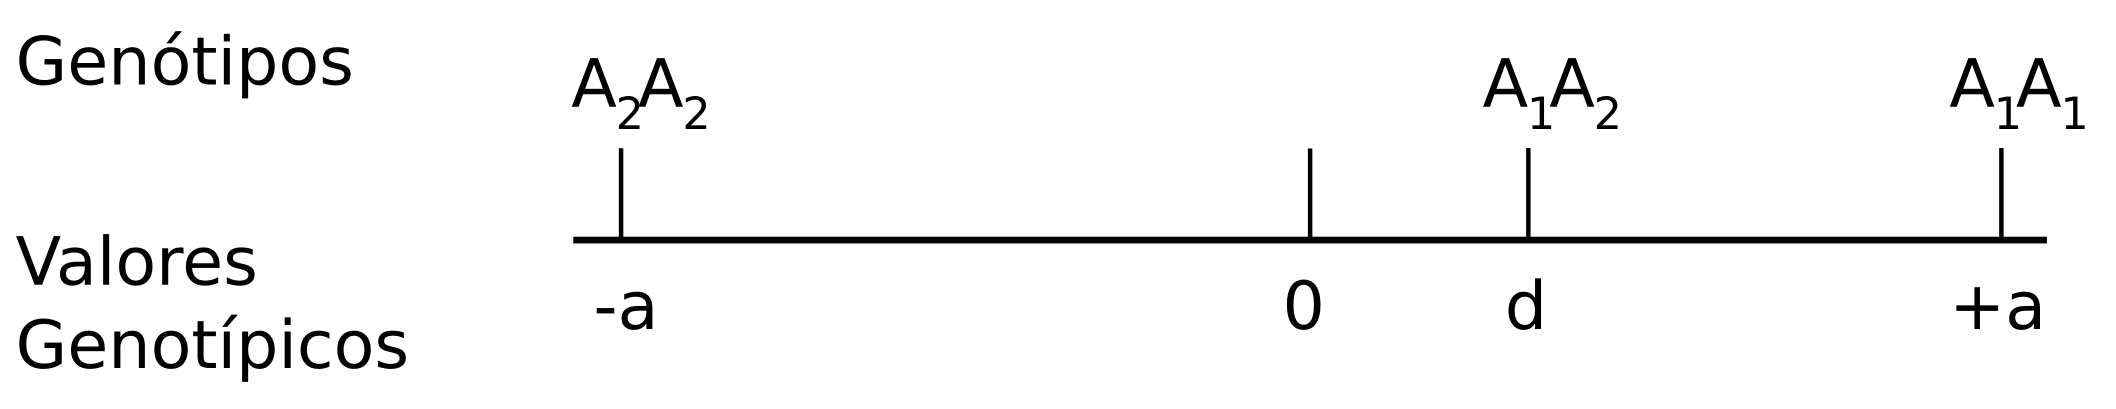
\includegraphics{./figuras/valoresgenotipicos.png}
\caption{Valores genotípicos arbitrários. O valor intermediário
entre os dois homozigotos foi denominado como zero. Os valores
genotípicos \(a\), \(-a\) e \(d\) são calculados em relação a esse ponto
zero.}
\label{valgen}
\end{marginfigure}

Portanto, ao medirmos uma amostra de indivíduos de uma população
qualquer, e, conhecendo seus genótipos, podemos chegar nos seus valores
genotípicos correspondentes. Por exemplo, digamos que o gene P, com dois
alelos, determine o peso em uma determinada população de ratos, e ao
pesarmos uma amostra encontramos: \(P_1\)\(P_1\) = 14g; \(P_1\)\(P_2\) =
12g; e \(P_2\)\(P_2\) = 6g. Então, para calcularmos o ponto zero, temos
que achar o valor intermediário entre os dois homozigotos:
\((14 + 6)/2 = 10\). Sendo 10g o ponto zero, o valor de a é:
\(14-10 = 4g\); o valor de -a é: \(6-10 = -4g\); e o valor de d é:
\(12-10 = 2g\).

Uma questão fundamental a se compreender sobre os valores genotípico e
fenotípico é que suas médias populacionais dependem das frequências
gênicas. Considerando a população em equilíbrio de Hardy-Weinberg
(acasalamento aleatório em relação aos loci em questão), podemos
calcular o valor médio populacional de um determinado caráter
determinado por um único locus multiplicando as frequências genotípicas
pelos valores genotípicos e somando os resultados para os três genótipos
(Tabela 1).

\begin{table}
  \centering
  \fontfamily{ppl}\selectfont
  \caption{Dependência da média populacional das frequências
gênicas. A frequência dos genótipos é determinada pelo equilíbrio
de Hardy-Weinberg e os valores genotípicos são calculados em relação
ao ponto equidistante dos dois homozigotos.}
  \begin{tabular}{llll}
    \toprule
  Genótipo  &  Frequência   &  Valor   &   Freq. $\times$ Valor \\
    \midrule
 $A_1A_1$   &       $p^2$   &        +a &        $p^2a$ \\
 $A_1A_2$   &       $2pq$   &         d &        $2pqd$ \\
 $A_2A_2$   &       $q^2$   &        -a &        $-q^2a$ \\
            &               &   soma =  &   $a(p-q)+2dpq$ \\
    \bottomrule
  \end{tabular}
\end{table}

Podemos ver, então, que a contribuição de qualquer locus para a média
populacional tem dois termos: \(a(p-q)\) atribuído aos homozigotos, e
\(2dpq\) atribuído aos heterozigotos. Se o alelo \(A_1\) fosse fixado na
população (\(p = 1\)), a média populacional seria a; se o alelo \(A_2\)
fosse fixado (\(q = 1\)), a média seria -a. Vamos voltar ao exemplo do
gene P, que determina o peso nos ratos, e calcular a média populacional.
Digamos que a frequência de \(P_1\) seja \(p = 0,6\), e lembrando que
\(a = 4\) e \(d = 2\), então:

\[
M = (0,6)^2 4 + 2(0,6)(0,4) 2 + (0,4)^2 -4 = 1,76g
\]

Se o caráter peso fosse determinado por mais de um locus, teríamos que
computar a contribuição de todos os loci e achar seu efeito combinado na
média populacional. Supondo que essa combinação é aditiva, ou seja, que
o efeito de um locus sobre a média é independente do efeito dos outros
loci, e que todos os loci sejam bialélicos, a média populacional será:

\[
M = \sum_{i}a_i(p_i-q_i) + 2d_ip_iq_i
\]

ou seja, a soma das médias de todos os loci.

\section{Efeito médio de um alelo}\label{efeito-muxe9dio-de-um-alelo}

Para entendermos a herança de caracteres quantitativos, temos que lidar
com a transmissão de valor dos pais para a prole. Isso não pode ser
feito somente com o uso dos valores genotípicos, pois os pais passam
seus genes e não seu genótipo para sua prole. O efeito médio de um alelo
é justamente uma medida associada com os genes e não com os genótipos.
Essa medida depende dos valores genotípicos, \(a\) e \(d\), e, também,
das frequências gênicas. Trata-se, portanto, de uma propriedade não só
dos genes, mas também da população. O efeito médio de um alelo
particular é o valor médio dos indivíduos que receberam esse alelo de um
dos pais descontado da média populacional, sendo o outro alelo
proveniente ao acaso da população (Tabela 2). Dito de uma outra maneira:
vamos considerar um número de gametas carregando o alelo \(A_1\)
unindo-se ao acaso com gametas da população. O genótipo médio produzido
desvia da média populacional por uma quantidade que é o efeito médio do
alelo \(A_1\). A dependência do efeito médio de um alelo das frequências
gênicas está na junção ao acaso do alelo específico com os provenientes
da população. A chance desse alelo se unir a um outro qualquer é
determinada pelas frequências gênicas desses outros alelos na população.

\newpage

\textbf{Tabela 2 }. Efeito médio dos alelos \(A_1\) e \(A_2\). Cada
gameta pode produzir dois genótipos distintos (homozigoto e
heterozigoto) conforme as frequências dos outros gametas na população.
Somando-se os valores genotípicos multiplicados por suas frequências e
descontando a média populacional, obtemos os efeitos médios dos alelos
\(A_1\) e \(A_2\).

\begin{table}
\begin{tabular}{lllllll}
\hline
& & & & & \\
Tipo de & \multicolumn{3}{l} {Valores e Freq.} & Valor médio & Média populacional & Efeito médio \\
gameta & \multicolumn{3}{l} {dos genótipos} & dos genótipos & a ser descontada & do alelo \\
 & \multicolumn{3}{l} { produzidos } & produzidos & & \\
& & & & & \\
\cline{2-4}
& & & & & \\
 & $A_1$$A_1$ & $A_1$$A_2$ & $A_2$$A_2$ & & \\
 & $a$ & $d$ & $-a$ & & \\
& & & & & \\
\hline
& & & & & \\
$A_1$ & $p$ & $q$ & & $pa + qd$ & $-[a(p-q) + 2dpq]$ & $q[a+d(q-p)]$ \\
$A_2$ & & $p$ & $q$ & $-qa + pd$ & $-[a(p-q) + 2dpq]$ & $-p[a+d(q-p)]$ \\
& & & & & \\
\hline

\end{tabular}
\end{table}

O efeito médio de um alelo é representado pelo símbolo \(\alpha_1\),
para o alelo \(A_1\), e \(\alpha_2\) para o alelo \(A_2\). Quando
trabalhamos com apenas dois alelos, podemos também calcular o efeito
médio da substituição de um alelo. Isso significa que se todos os genes
\(A_2\) fossem mutados para o gene \(A_1\), o efeito médio produzido
será o efeito médio da substituição, representado pelo símbolo
\(\alpha\): \[
\alpha = a + d(q-p)
\] O valor de \(\alpha\) é obtido seguindo o raciocínio de que ao
mudarmos o genótipo \(A_1A_2\) pelo genótipo \(A_1A_1\), mudaremos o
valor d para o +a, e o efeito será \((a - d)\). Ao mudarmos \(A_2A_2\)
para \(A_1A_2\), mudaremos o valor de -a para d, e o efeito será
\((d + a)\).

\section{Valor de acasalamento}\label{valor-de-acasalamento}

Os efeitos médios de todos os alelos parentais influenciando um caráter
determinam o valor genotípico médio de sua prole para esse caráter.
Porém, é impossível medir o efeito médio de cada alelo nos indivíduos,
pois os efeitos médios são propriedades populacionais, envolvendo a
associação de cada alelo com todas a diferentes combinações genéticas
possíveis em cada indivíduo. Felizmente, o que podemos medir é o valor
de acasalamento (simbolizado pela letra A): o valor fenotípico de um
indivíduo julgado pelo valor médio do caráter em sua prole. Ou seja,
podemos pegar um indivíduo e realizar cruzamentos com outros indivíduos
sorteados da população e tirar a média do valor fenotípico do caráter em
sua prole. Se um indivíduo se reproduz com um número de parceiros
retirados ao acaso da população, seu valor de acasalamento é duas vezes
o desvio médio de sua prole da média populacional. É necessário
multiplicar por dois pois o pai em questão passa somente metade dos seus
genes a sua prole, a outra metade vindo ao acaso da população. Essa é a
definição prática de valor de acasalamento, o valor que os pais
efetivamente passam à sua prole. No entanto, pela teoria, assumimos que
o valor de acasalamento é na verdade a soma dos efeitos médios de todos
os alelos que um indivíduo carrega. O valor de acasalamento, portanto,
pode ser expresso em termos dos efeitos médios dos alelos (ou efeito
médio de uma substituição de alelo), como mostrado na tabela 3.

\begin{margintable}
  \centering
  \fontfamily{ppl}\selectfont
  \caption{Valores de acasalamento para os genótipos de um locus com
dois alelos. O valor de acasalamento está apresentado em função dos
efeitos médios dos alelos ($\alpha_1$ e $\alpha_2$) e do efeito médio
de uma substituição ($\alpha$).}
  \begin{tabular}{ll}
    \toprule
Genótipo &   Valor de acasalamento \\
    \midrule
$A_1$$A_1$ & $2\alpha_1 = 2q\alpha$ \\
$A_1$$A_2$ & $\alpha_1 + \alpha_2 = (q-p)\alpha$ \\
$A_2$$A_2$ & $2\alpha_2 = -2p\alpha$ \\
    \bottomrule
  \end{tabular}
\end{margintable}

A extensão para vários loci é direta: o valor de acasalamento para um
genótipo particular é a soma dos valores de acasalamento atribuídos a
cada loci separado (assumindo que os efeitos dos alelos são aditivos).

\section{Desvio de dominância}\label{desvio-de-dominuxe2ncia}

O valor de acasalamento é componente aditivo do valor genotípico de um
indivíduo. O restante do valor genotípico é denominado desvio de
dominância:

\[
G = A + D
\]

\begin{marginfigure}
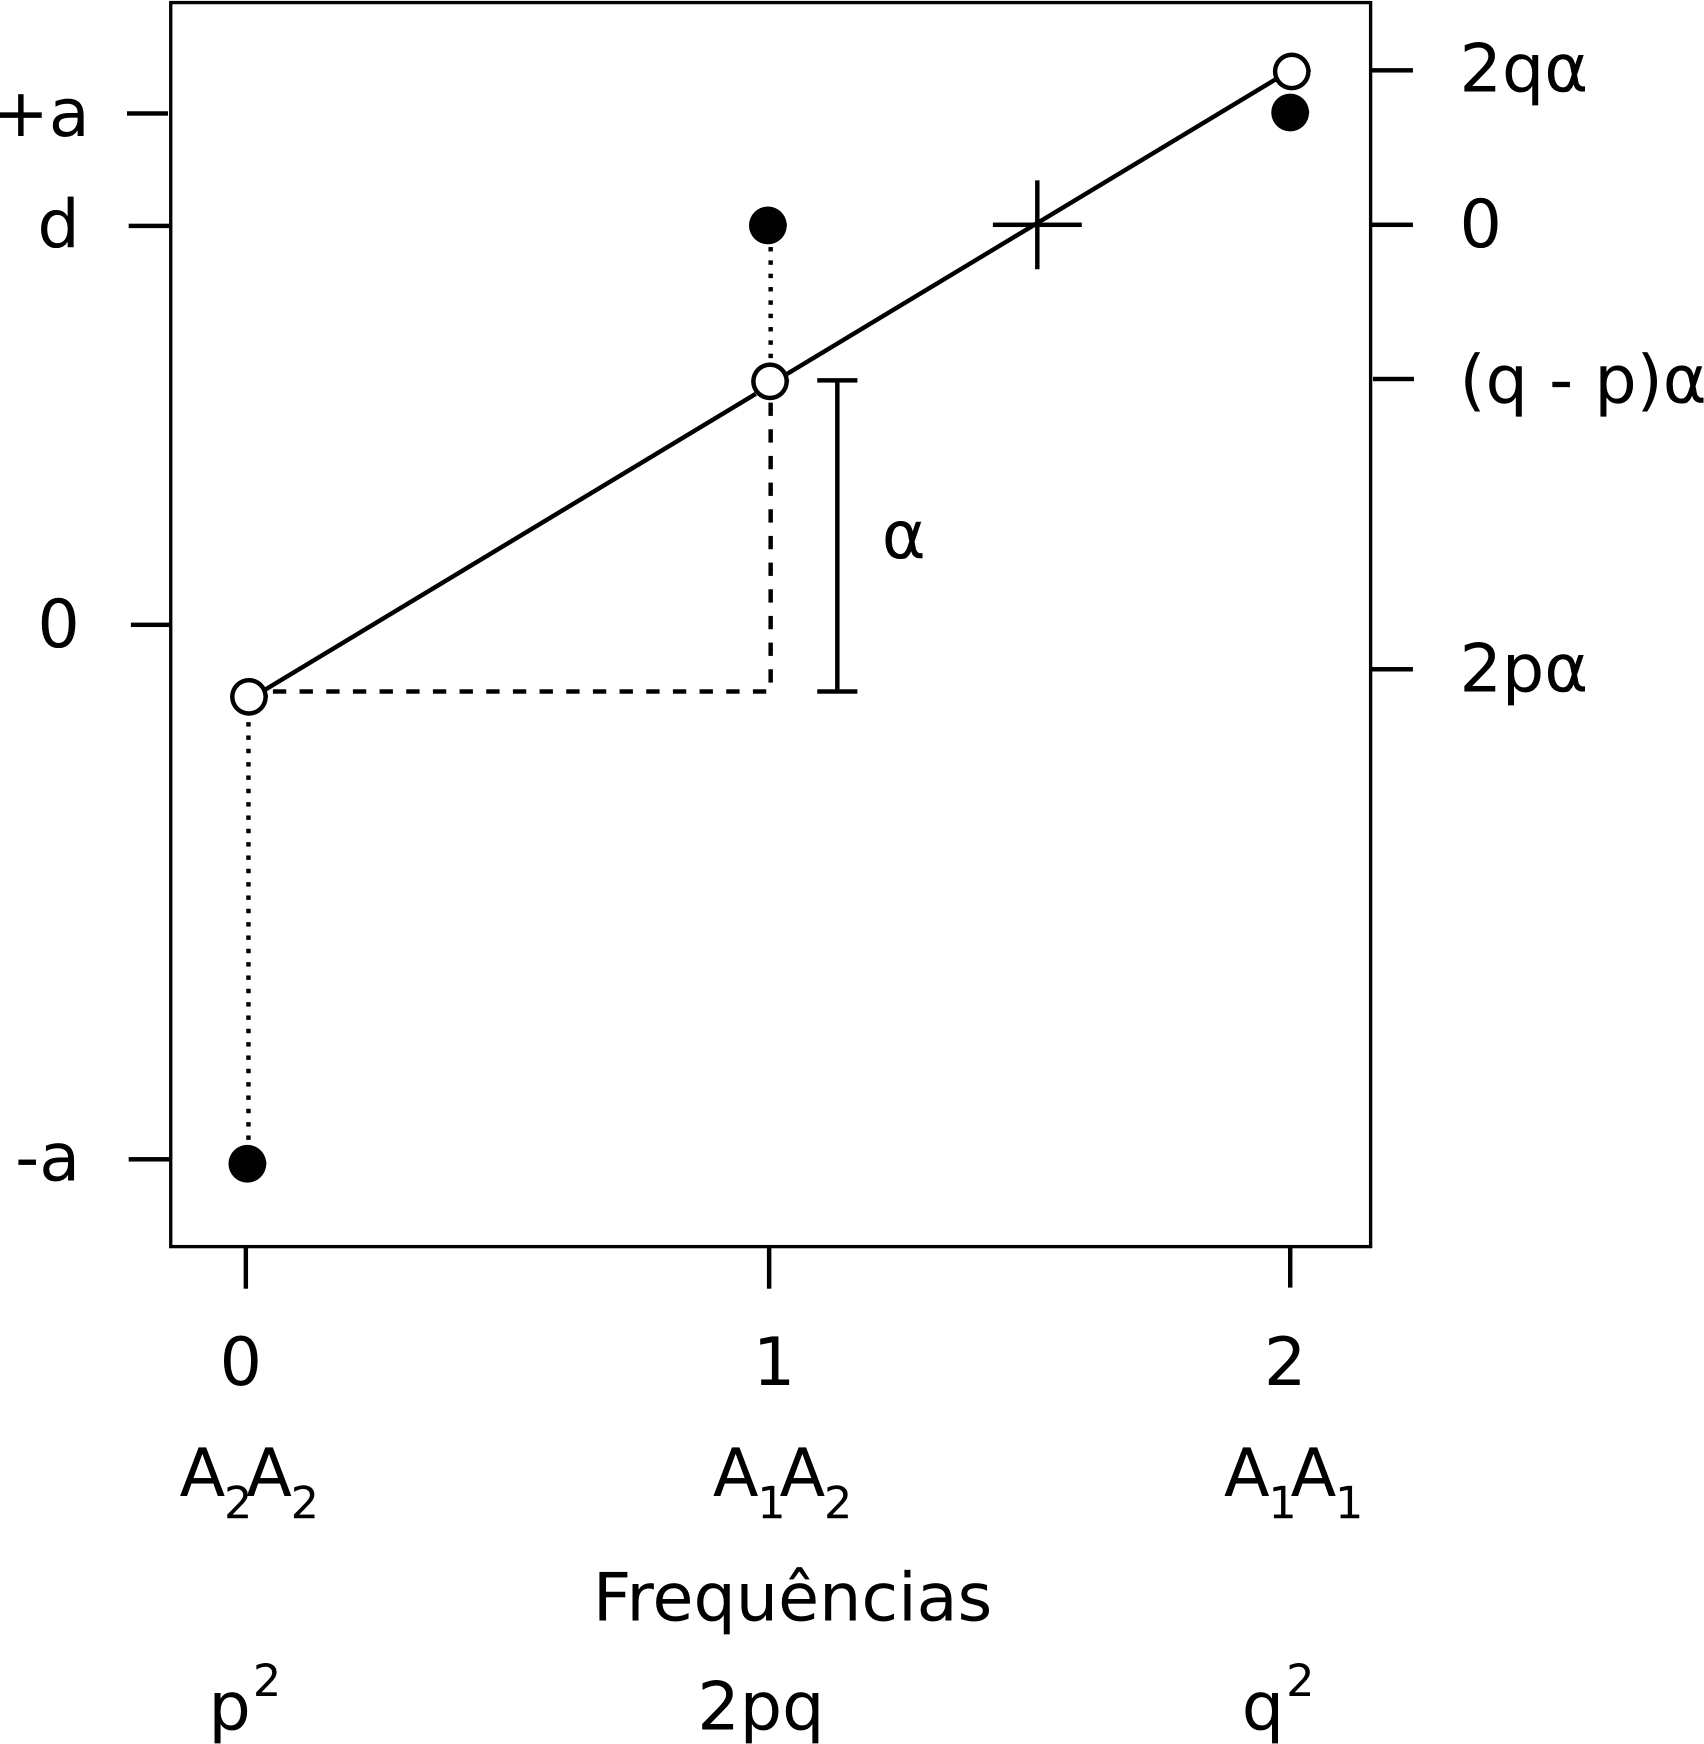
\includegraphics{./figuras/desviodominancia.png}
\caption{Valores genotípicos, valores de acasalamento e desvios
de dominância para um locus com dois alelos. Os círculos abertos
representam os valores de acasalamento para os genótipos apresentados no
eixo da abscissa. Esse eixo indica o número de alelos \(A_1\) no
genótipo. Os círculos preenchidos representam os valores genotípicos
observados. Os desvios de dominância são as linhas pontilhadas que
conectam os valores de acasalamento com os valores genotípicos. A cruz
representa a média populacional. O eixo vertical à esquerda mostra os
valores genotípicos, enquanto o eixo à direita mostra os valores de
acasalamento correspondentes aos genótipos na abscissa.}
\label{desviodominancia}
\end{marginfigure}

Esse desvio tem origem na propriedade de dominância entre alelos de um
mesmo locus, ou seja, na interação dentro do locus. O desvio de
dominância, portanto, aparece quando os alelos são unidos para formar um
genótipo. Esse efeito não pode ser previsto pelos efeitos dos alelos
separadamente. Dado que os efeitos médios dos alelos e os valores
genotípicos dependem da frequência gênica, o desvio de dominância também
possuí essa dependência, sendo uma propriedade tanto dos genes quanto da
população. A relação entre valores genotípicos, valores de acasalamento
e desvios de dominância está representada graficamente na figura
\ref{desviodominancia}. Nesta figura, os valores genotípicos estão
plotados contra o número de alelos \(A_1\) no genótipo. Uma reta de
regressão pelo método de quadrados mínimos está ajustada aos valores
genotípicos e os pontos apresentam pesos conforme a frequência do
genótipo que ele representa. A posição dessa reta dá os valores de
acasalamento de cada genótipo. As diferenças entre valores de
acasalamento e valores genotípicos correspondem aos desvios de
dominância.

\section{Desvio de interação}\label{desvio-de-interauxe7uxe3o}

Quando apenas um locus é considerado, apenas o efeito da interação entre
os alelos desse locus é adicionado ao valor de acasalamento para a
determinação do valor genotípico. Porém, quando mais loci são
considerados, o valor genotípico pode ter um componente a mais, o desvio
de interação, relacionado com a interação entre alelos de diferentes
loci (epistasia):

\[
G = A_A + D_A + A_B + D_B + I_{AB}
\]

\(I_{AB}\) é o desvio da combinação aditiva dos valores genotípicos
\(G_A\) e \(G_B\), o desvio epistático. Interações epistáticas são
fundamentais na formação de associações gênicas funcionais e modulares,
como veremos nas próximas seções. Além disso, epistasia pode funcionar
como uma forma de armazenar variação críptica, liberada em eventos
seletivos intensos ou gargalos populacionais \cite{Cheverud1996a}.

\section{Partição de variância}\label{partiuxe7uxe3o-de-variuxe2ncia}

Valores genotípicos, fenotípicos e de acasalamento e desvios de
dominância e de interação são medidas associadas a indivíduos. Porém,
quando lidamos com a evolução de populações, usamos a combinação dessas
quantidades expressada em termos de variação em torno da média. Como
vimos anteriormente, a variação dos caracteres contínuos é expressa em
termos de variância. A ideia básica no estudo de variação, introduzida
por Fisher \cite{Fisher1918}, é de sua partição em componentes
atribuídos a diferentes causas. A magnitude relativa desses componentes
determina as propriedades genéticas de uma população, em particular o
grau de semelhança entre parentes. Os componentes nos quais a variância
é particionada são os mesmos nos quais o valor fenotípico foi dividido:

\[
V_P = V_A + V_D + V_I + V_E
\]

sendo \(V_P\) a variância dos valores fenotípicos, \(V_A\) a variância
dos valores de acasalamento (chamada de variância aditiva), \(V_D\) a
variância dos desvios de dominância, \(V_I\) a variância dos desvios
epistáticos, e finalmente \(V_E\) a variância dos desvios ambientais. A
importância relativa de uma determinada fonte de variação é a variância
devida a essa fonte, como uma proporção da variância fenotípica.

\section{Variância aditiva}\label{variuxe2ncia-aditiva}

A variância aditiva, ou a variância devida aos valores de acasalamento,
é a causa principal de semelhança entre parentes, sendo, portanto, o
determinante das propriedades genéticas da população e de sua resposta à
seleção natural. A razão \(V_A/V_P\) expressa a extensão na qual os
fenótipos são determinados pelos genes transmitidos pelos pais, e é
denominada herdabilidade.

\section{Seleção Natural e Genética
Quantitativa}\label{seleuxe7uxe3o-natural-e-genuxe9tica-quantitativa}

Agora que fizemos a conexão entre efeito médio dos alelos, valor de
acasalamento, variância aditiva e herdabilidade, podemos estudar a
resposta à seleção natural de um caráter ou de vários caracteres
simultaneamente. As propriedades genéticas de uma população são um
produto da seleção natural que atuou no passado, junto de mutação,
recombinação e deriva genética. É por meio desses processos que existe
variabilidade genética, e é principalmente pela ação da seleção natural
que os caracteres diferem, alguns tendo proporcionalmente mais variação
genética aditiva que outros. A teoria da genética quantitativa fornece
duas equações pelas quais poemos compreender a resposta à seleção
natural em um único caráter - Equação do Criador - e de vários
caracteres simultaneamente - Equação de Lande.

\section{Um caráter: Equação do
Criador}\label{um-caruxe1ter-equauxe7uxe3o-do-criador}

Quando estamos trabalhando com apenas um caráter, podemos calcular sua a
resposta à seleção natural (R) conforme o diferencial de seleção
aplicado (S) e a herdabilidade (\(h^2\)) desse caráter. Essa resposta
univariada à seleção natural foi nomeada como Equação do Criador
(``Breeder's equation''), em referência a criadores de animais e de
plantas que aplicavam seleção artificial com intuito de atingir maior
produtividade:

\[
R = h^2S
\]

Nessa equação, podemos notar a relevância da herdabilidade, ou da
proporção de variância devida aos valores de acasalamento, na
determinação da resposta à seleção natural. Quanto maior for essa
proporção, maior será a resposta à seleção para um mesmo diferencial de
seleção.

\section{Médias}\label{muxe9dias}

Apesar de um episódio de seleção alterar as frequências alélicas do
caráter, os efeitos da seleção passíveis de observação restringem-se às
mudanças mensuradas na média da população. Portanto, a resposta à
seleção (R) é uma diferença entre as médias fenotípicas do caráter na
prole dos pais selecionados e na geração parental antes da seleção.

\section{Diferencial de Seleção}\label{diferencial-de-seleuxe7uxe3o}

O diferencial de seleção é definido como a diferença na média dos
indivíduos selecionados e a média populacional antes da seleção. Na
figura \ref{parentoff} podemos ver um evento de seleção de truncamento,
ou seja, apenas indivíduos com fenótipo acima de um certo valor
sobrevivem. O diferencial de seleção \(S\) está relacionado com a
intensidade de seleção, quando maior o \(S\) mais intensa é a seleção.
Como o diferencial de seleção é expresso na escala da medida original,
podemos padronizá-lo pelo desvio padrão fenotípico. A quantidade
resultante é usualmente chamada de intensidade de seleção (\(i\)) e é
adimensional.

\[
\frac{S}{\sigma_P} = i
\]

\begin{marginfigure}
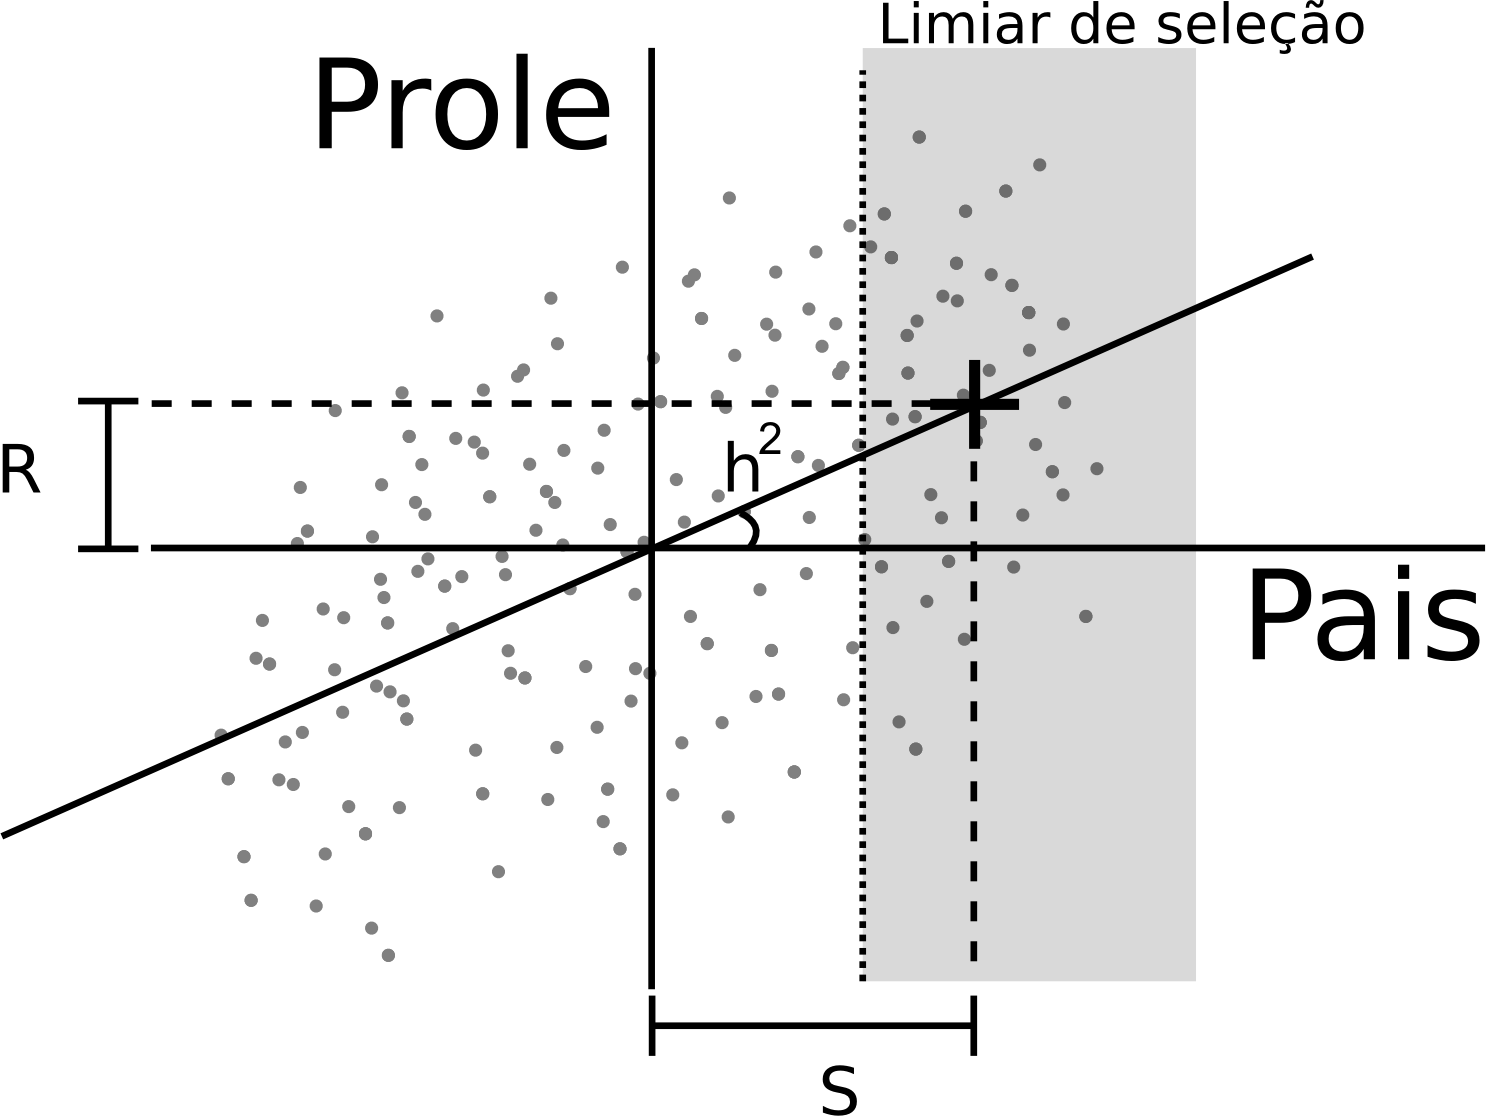
\includegraphics{./figuras/parent-offspring.png}
\caption{Resposta à seleção ilustrada na regressão dos resíduos
em torno da média do caráter dos pais pelos resíduos da prole. Cada
ponto é um par dos desvios do caráter dos pais e de sua prole em relação
à média populacional. A origem do gráfico (0,0) representa a média
populacional e assume-se que é a mesma nas duas gerações. A área
sombreada representa os indivíduos da geração parental que foram
selecionados. A cruz é a média dos pais e da prole selecionados. A
diferença da origem (média populacional) para a média dos pais
selecionados corresponde ao diferencial de seleção (S). A diferença da
origem para a média da prole corresponde à resposta à seleção (R).}
\label{parentoff}
\end{marginfigure}

\section{Herdabilidade}\label{herdabilidade}

Olhando para a regressão pais-prole da figura \ref{parentoff}, podemos
ver que a razão R/S é equivalente à inclinação da reta de regressão. Na
Equação do Criador, podemos notar que essa razão corresponde à
herdabilidade do caráter em questão. Lembrando que herdabilidade
representa a proporção de variância aditiva em relação à variância
fenotípica, vemos que a seleção atua sobre variação fenotípica da
população, mas a resposta na próxima geração é proporcional à variação
aditiva dos pais, ou seja, proporcional à variação nos seus valores de
acasalamento. Quanto mais próxima de 1,0 for a inclinação da reta de
regressão pais-prole, maior a semelhança entre pais e prole (maior a
herdabilidade), e, portanto, mais eficiente a resposta à seleção.

\section{Mais de um caráter: Equação de
Lande}\label{mais-de-um-caruxe1ter-equauxe7uxe3o-de-lande}

Sabemos que, quando trabalhamos com mais de um caráter, temos que
considerar não somente a variância dos caracteres, mas também a
covariância ou a correlação dos mesmos. A principal causa genética de
covariação entre caracteres é o padrão pleiotrópico dos genes, ou seja,
um gene afetando dois ou mais caracteres ao mesmo tempo. Portanto, se um
gene pleiotrópico está segregando na população, isso causa variação
correlacionada nos caracteres que ele afeta. Por exemplo, genes que
aumentam a taxa de crescimento de indivíduos aumentam tanto a altura
quanto o peso destes, causando uma correlação genética entre esses
caracteres. A intensidade da correlação genética entre dois caracteres
indica a força da associação genética herdável entre eles. O padrão de
pleiotropia está relacionado com o sistema de desenvolvimento dos
organismos, ou seja, caracteres que compartilham uma mesma via de
desenvolvimento, e com o desempenho de uma determinada função,
garantindo a coesão dos caracteres. Isso será melhor explicado na
próxima seção de Modularidade e Integração Morfológica.

Paralelo aos efeitos genéticos, a seleção natural atua em vários
caracteres simultaneamente, e a associação genética entre esses
caracteres pode alterar a resposta à seleção natural
\cite{Lande1983a}. A correlação entre caracteres causa uma resposta
indireta: se X e Y são correlacionados, a seleção direta em X causará
uma seleção correlacionada em Y, e uma resposta direta de X e indireta
de Y. Como vimos na Equação do Criador, a resposta direta de X é
proporcional à variância nos valores de acasalamento dos indivíduos
selecionados. Já a resposta indireta de Y pode ser prevista quando
conhecemos o valor da correlação genética entre X e Y e as
herdabilidades dos dois caracteres. A expansão da equação univariada
para a multivariada foi elaborada por Russel Lande \cite{Lande1979}.
A equação de resposta multivariada à seleção direcional é análoga à
equação do criador, e pode ser escrita como:

\[
\Delta z = GP^{-1}S = G\beta
\]

Onde \(\Delta z\) representa mudança na média entre duas gerações após
um evento de seleção na geração parental; \(\mathbf{G}\) representa a
matriz de covariância genética aditiva, ou seja, a matriz de covariância
dos efeitos médios dos alelos para cada um dos caracteres em questão;
\(P^{-1}\) representa a inversa da matriz de covariância fenotípica da
população; e, finalmente, \(S\) representa o vetor do diferencial de
seleção, ou seja, a diferença na média dos individuos parentais
selecionados e a média populacional antes da seleção. O poduto
\(P^{-1}S\) também é chamado de gradiente de seleção, ou \(\beta\).
Vamos detalhar individualmente cada uma dessas quantidades.

\section{Vetor de Resposta à Seleção \(\cdot\)
\(\Delta z\)}\label{vetor-de-resposta-uxe0-seleuxe7uxe3o-cdot-delta-z}

Como agora estamos trabalhando com vários caracteres, nossa
representação passa a ser vetorial. Cada entrada do vetor de médias de
uma população representa a média de um caráter. O vetor \(\Delta z\),
portanto, é somente a diferença nas médias de duas gerações, após um
evento de seleção na geração parental. Ele é exatamente equivalente ao R
na equação do criador.

\section{Diferencial e Gradiente de Seleção \(\cdot\) S e
\(\beta\)}\label{diferencial-e-gradiente-de-seleuxe7uxe3o-cdot-s-e-beta}

O vetor \(S\) é análogo ao S da equação do criador, e representa a
difereça na média dos parentais antes e depois da seleção, mas agora
para todos os caracteres simultaneamente. No caso multivariado, os
diferenciais de seleção não são restritos ao caráter selecionado, pois,
caso haja covariação entre o caráter selecionado e um segundo caráter
não selecionado, um diferencial de seleção indireto se manifesta (Fig.
\ref{difsel}):

\begin{marginfigure}
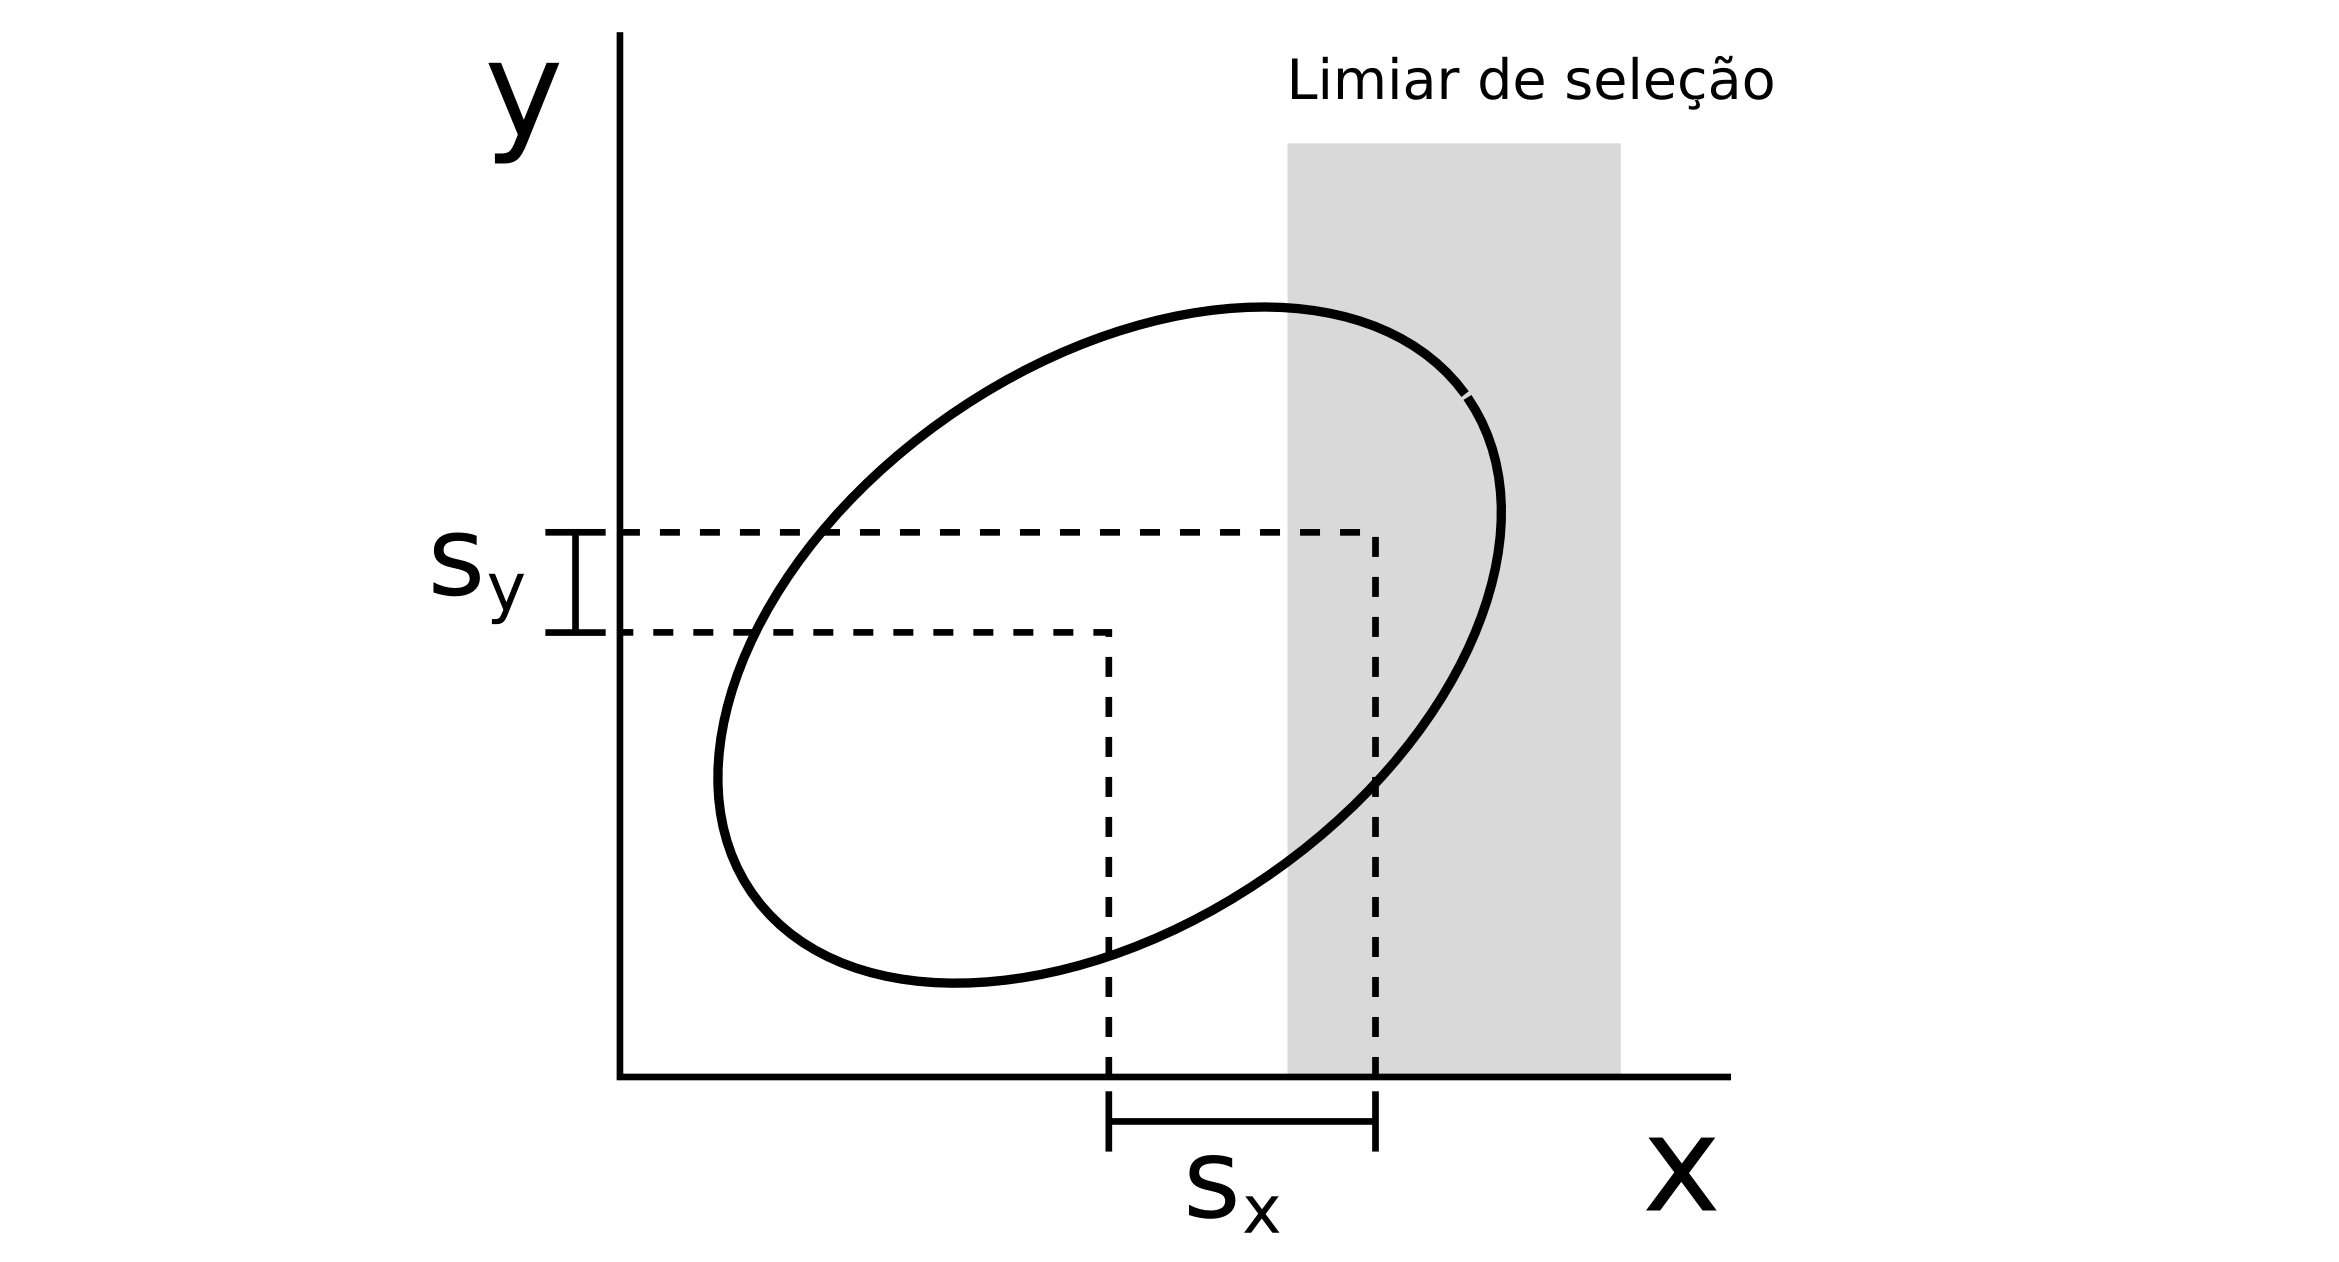
\includegraphics{./figuras/diferencialdeselecao.png}
\caption{Diferencial de seleção correlacionado Apenas o caráter
\(X\) está sujeito à seleção de truncamento, porém vemos um diferencial
correlacionado em \(Y\), devido à covariação fenotípica entre as duas
variáveis. A elipse representa um intervalo de confiança de 95\% da
distribuição fenotípica das duas variáveis.}
\label{difsel}
\end{marginfigure}

Podemos, então, descontar a correlação fenotípica encontrada na
população para obter um valor de seleção que seja apenas devido a
seleção direta em cada caráter.

Isso é feito multiplicando o diferencial de seleção pelo inverso da
matriz de covariação fenotípica, obtendo o gradiente de seleção (Fig.
\ref{gradsel}). O vetor resultante, \(\beta\), representa apenas a
seleção direta em cada caráter, em unidades de variância fenotípica.

\begin{marginfigure}
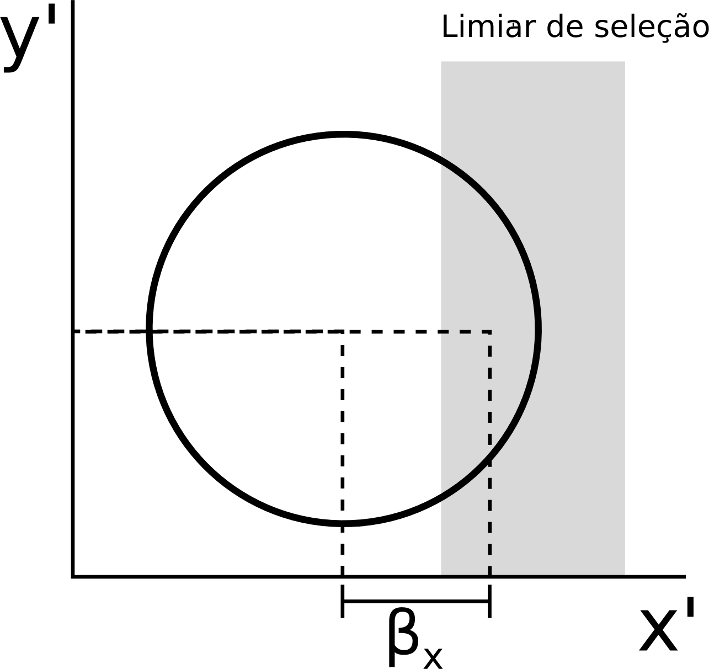
\includegraphics{./figuras/gradientedeselecao.png}
\caption{Gradiente de seleção correlacionado. A partir da
situação na figura \ref{difsel}, descontamos o efeito da covariação
fenotípica entre duas variáveis e obtemos os gradientes de seleção. Como
não existe seleção direta sobre $y$, sua componente do gradiente de
seleção é nula.}
\label{gradsel}
\end{marginfigure}

\section{Matriz Genética}\label{matriz-genuxe9tica}

A matriz genética ou \(\mathbf{G}\) possuí como entradas em sua diagonal
os valores de variância aditiva (\(V_A\)) para cada caráter, que é o
numerador do cálculo de herdabilidade (\(h^2 = V_A/V_P\)). Ou seja, a
diagonal da \(\mathbf{G}\) determina as respostas diretas dos caracteres
ao gradiente de seleção. Fora das diagonais, as entradas são as
covariâncias genéticas aditivas entre todos os caracteres considerados,
que determinam as respostas indiretas dos mesmos.

Para entender melhor o efeito das correlações genéticas na resposta à
seleção, vamos olhar para a equação de Lande no caso de 3 caracteres e
abrir o produto do gradiente de seleção com a matriz \(\mathbf{G}\) em
todos os seus termos.

\begin{align}
\mathbf{G}\beta  =
\left (
\begin{matrix}
G_{11} & G_{12} & G_{13}\\
G_{21} & G_{22} & G_{23} \\
G_{31} & G_{32} & G_{33}\\
\end{matrix}
\right )
\left (
\begin{matrix}
\beta_{1}  \\
\beta_{2}   \\
\beta_{3}  \\
\end{matrix}
\right )
&=
\left (
\begin{matrix}
G_{11}\beta_{1} +  G_{12}\beta_{2} +  G_{13}\beta_{3}\\
G_{21}\beta_{1} +  G_{22}\beta_{2} +  G_{22}\beta_{3}\\
G_{31}\beta_{1} +  G_{32}\beta_{2} +  G_{32}\beta_{3}\\
\end{matrix}
\right )
\\
&=
\left (
\begin{matrix}
\Delta z_{1}  \\
\Delta z_{2}   \\
\Delta z_{3}  \\
\end{matrix}
\right )
=
\Delta z
\end{align}

Os termos \(G_{11}\beta_{1}\), \(G_{22}\beta_{2}\) e \(G_{33}\beta_{3}\)
representam a resposta à seleção direta em cada caráter. Mas, vemos que,
além dos termos diretos, temos também todos os termos indiretos, que são
termos de resposta correlacionada devido à covariação genética entre os
caracteres. Ou seja, o efeito que a seleção em um caráter provoca em
todos os outros que estão correlacionados com ele. A presença de
respostas indiretas a um dado gradiente de seleção faz com a resposta
observada (\(\Delta z\)) não seja na mesma direção que o vetor de
seleção. Esse desvio da direção de seleção foi denominado restrição
evolutiva (fig. \ref{desvio-trajetorias}) Portanto, os componentes de
covariância da \(\mathbf{G}\) podem restringir a evolução de uma
população na direção da seleção, enquanto que os componentes de
variância aditiva podem restringir a taxa de evolução, no caso de pouca
variância. Apesar da relevância da \(\mathbf{G}\) em evolução, sua
estimativa não é uma tarefa simples, pois são necessários delineamentos
de cruzamento entre os indivíduos de uma população e criação de sua
prole para a determinação do parentesco entre eles (pais-filhos, irmãos,
meio-irmãos).

\begin{figure}
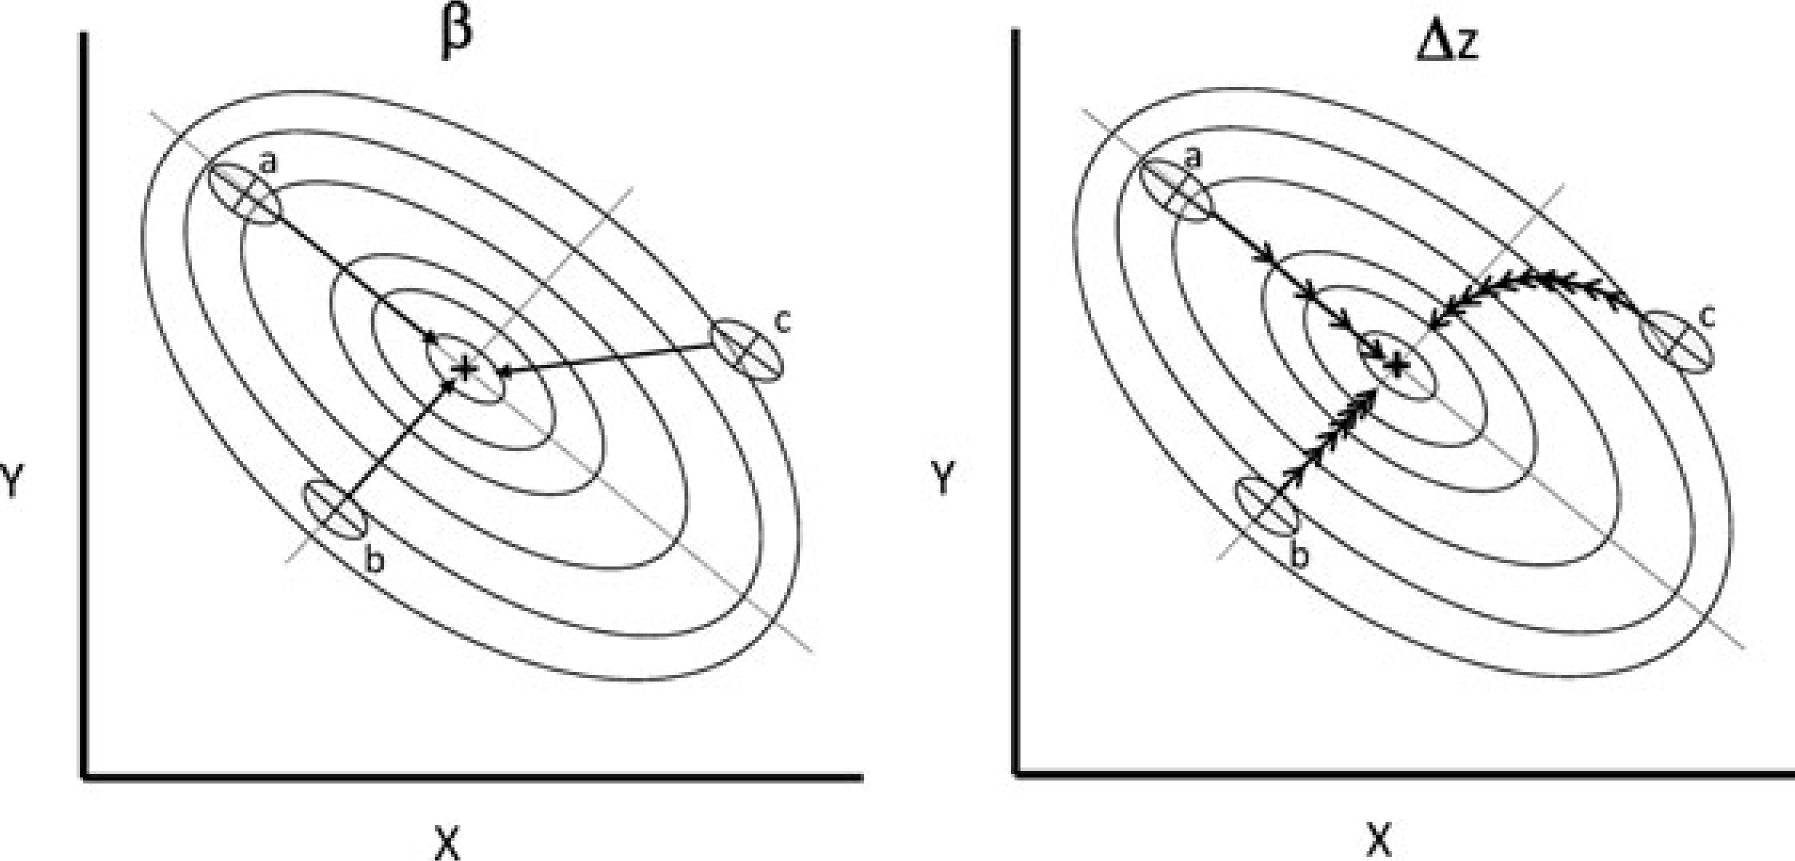
\includegraphics{./figuras/desvio-trajetorias.png}
\caption{Trajetórias evolutivas de populações com estruturas de
covariação orientadas de formas distintas na paisagem adaptativa. Estão
apresentadas três matrizes G (elipses cinzas) dispostas em uma paisagem
adaptativa, na qual as elipses concêntricas reperesentam diferentes
valores de aptidão. A cruz ao centro da paisagem indica o ótimo
adaptativo, e portanto a direção para qual as matrizes são puxadas pela
seleção. As matrizes \emph{a} e \emph{b} respondem de maneira linear
(sem desvios) à seleção, pois possuem um de seus eixos de variação
alinhados com a paisagem. Já a matriz \emph{c}, que não está alinhada
com a paisagem, apresenta uma resposta curva à seleção, ou seja, sua
trajetória evolutiva está restringida pela sua estrutura de covariância
genética aditiva.}
\label{desvio-trajetorias}
\end{figure}

\section{Matriz Fenotípica}\label{matriz-fenotuxedpica}

A matriz P é muito mais simples de ser obtida, pois não precisamos ter
acesso ao grau de parentesco entre os indivíduos amostrados. A
amostragem pode ser feita em indivíduos de coleções de museu, por
exemplo, e grandes amostras podem ser obtidas garantindo uma boa
estimativa da \(\mathbf{P}\). A \(\mathbf{P}\) é semelhante em seu
arranjo à \(\mathbf{G}\), apenas tendo no lugar das variâncias e
covariâncias genéticas aditivas, as variâncias e covariâncias
fenotípicas. Portanto, a \(\mathbf{P}\) contabiliza tanto os efeitos
genéticos aditivos quanto os ambientais. Mas, uma vez que a
\(\mathbf{G}\) reflete as relações entre caracteres determinadas pelo
desenvolvimento/função dos organismos, as variações ambientais devem
atuar pelas mesmas vias de desenvolvimento que as variações genéticas, e
portanto o padrão de correlações ambientais também deve refletir as
restrições de desenvolvimento \cite{Cheverud1984}. Sendo assim, as
correlações fenotípicas seriam similares às correlações genéticas. A
similaridade entre matrizes \(\mathbf{G}\) e \(\mathbf{P}\) foi testada
empiricamente em espécies de mamíferos por diferentes autores e
verificou-se que quando a matriz G é melhor estimada (ou seja, quando o
número de indivíduos amostrados é superior a 40), a similaridade com sua
matriz P correspondente é alta \cite{Cheverud1988}. A expectativa de
similaridade entre \(\mathbf{G}\) e \(\mathbf{P}\) é denominada
``Conjectura de Cheverud'', pois foi esse autor que a propôs e a testou
em primeiro lugar. Portanto, dada a Conjectura de Cheverud, podemos
substituir as matrizes G das espécies por suas respectivas matrizes P e
realizar estudos macro-evolutivos, isto é, podemos estudar a evolução de
caracteres ao longo de uma filogenia.

A Equação de Lande pode ser estendida para sua forma macro-evolutiva:

\[
\beta = G^{-1} (\overline z_{atual} - \overline z_{ancestral})
\]

na qual \((\overline z_{atual} - \overline z_{ancestral})\) representa a
diferença na média das espécies atuais e ancestrais, e o gradiente de
seleção \(\beta\) representa o padrão de seleção cumulativo sofrida por
cada linhagem independentemente \cite{Marroig2005}. A aplicação
dessa forma macro-evolutiva da Equação de Lande só pode ser feita se
existir constância da \(\mathbf{G}\) (ou, no caso, da \(\mathbf{P}\)).
Essa premissa está relacionada com homogeneidade de variâncias e
covariâncias genéticas aditivas entre as espécies estudadas e a
reconstrução de matrizes ancestrais dos nós mais internos da filogenia.

\section{Modularidade e
Integração}\label{modularidade-e-integrauxe7uxe3o}

Na imensa maioria dos organismos, conseguimos identificar partes
relativamente discretas e separadas, frequentemente envolvidas no
desempenho de alguma função. Em organismos unicelulares podemos
distinguir organelas desempenhando funções específicas, bem como regiões
internas ou na membrana responsáveis por processos distintos. Já nos
multicelulares, tipos celulares são organizados em tecidos espacialmente
separados, formando órgãos de funções distintas, que por sua vez são
organizados em sistemas responsáveis por funções distintas. Modularidade
se refere a esse padrão de organização dos seres vivos, onde algumas
partes são mais relacionadas entre si do que com outras partes do mesmo
organismo. Podemos descrever, e entender, a organização entre partes
constituintes dos organismos através das relações entre elas, sendo cada
tipo de relação adequada a um nível de complexidade ou organização. As
partes do organismo as quais nos referimos podem ser as bases
nitrogenadas de uma molécula de RNA, genes, proteínas, ou caracteres
morfológicos, como temos visto até agora \cite{Wagner2007}. Essas
relações podem ser medidas de diversas formas, como interação física
entre proteínas, padrões de expressão conjunta entre genes, ou, no nosso
caso, correlação entre caracteres quantitativos. Esse grupo de
características muito relacionadas entre si constituem um módulo, como
esquematizado na figura \ref{modulos}. Módulos, então, são
caracterizados por uma alta conectividade interna e relativa
independência de outros módulos.

\begin{marginfigure}
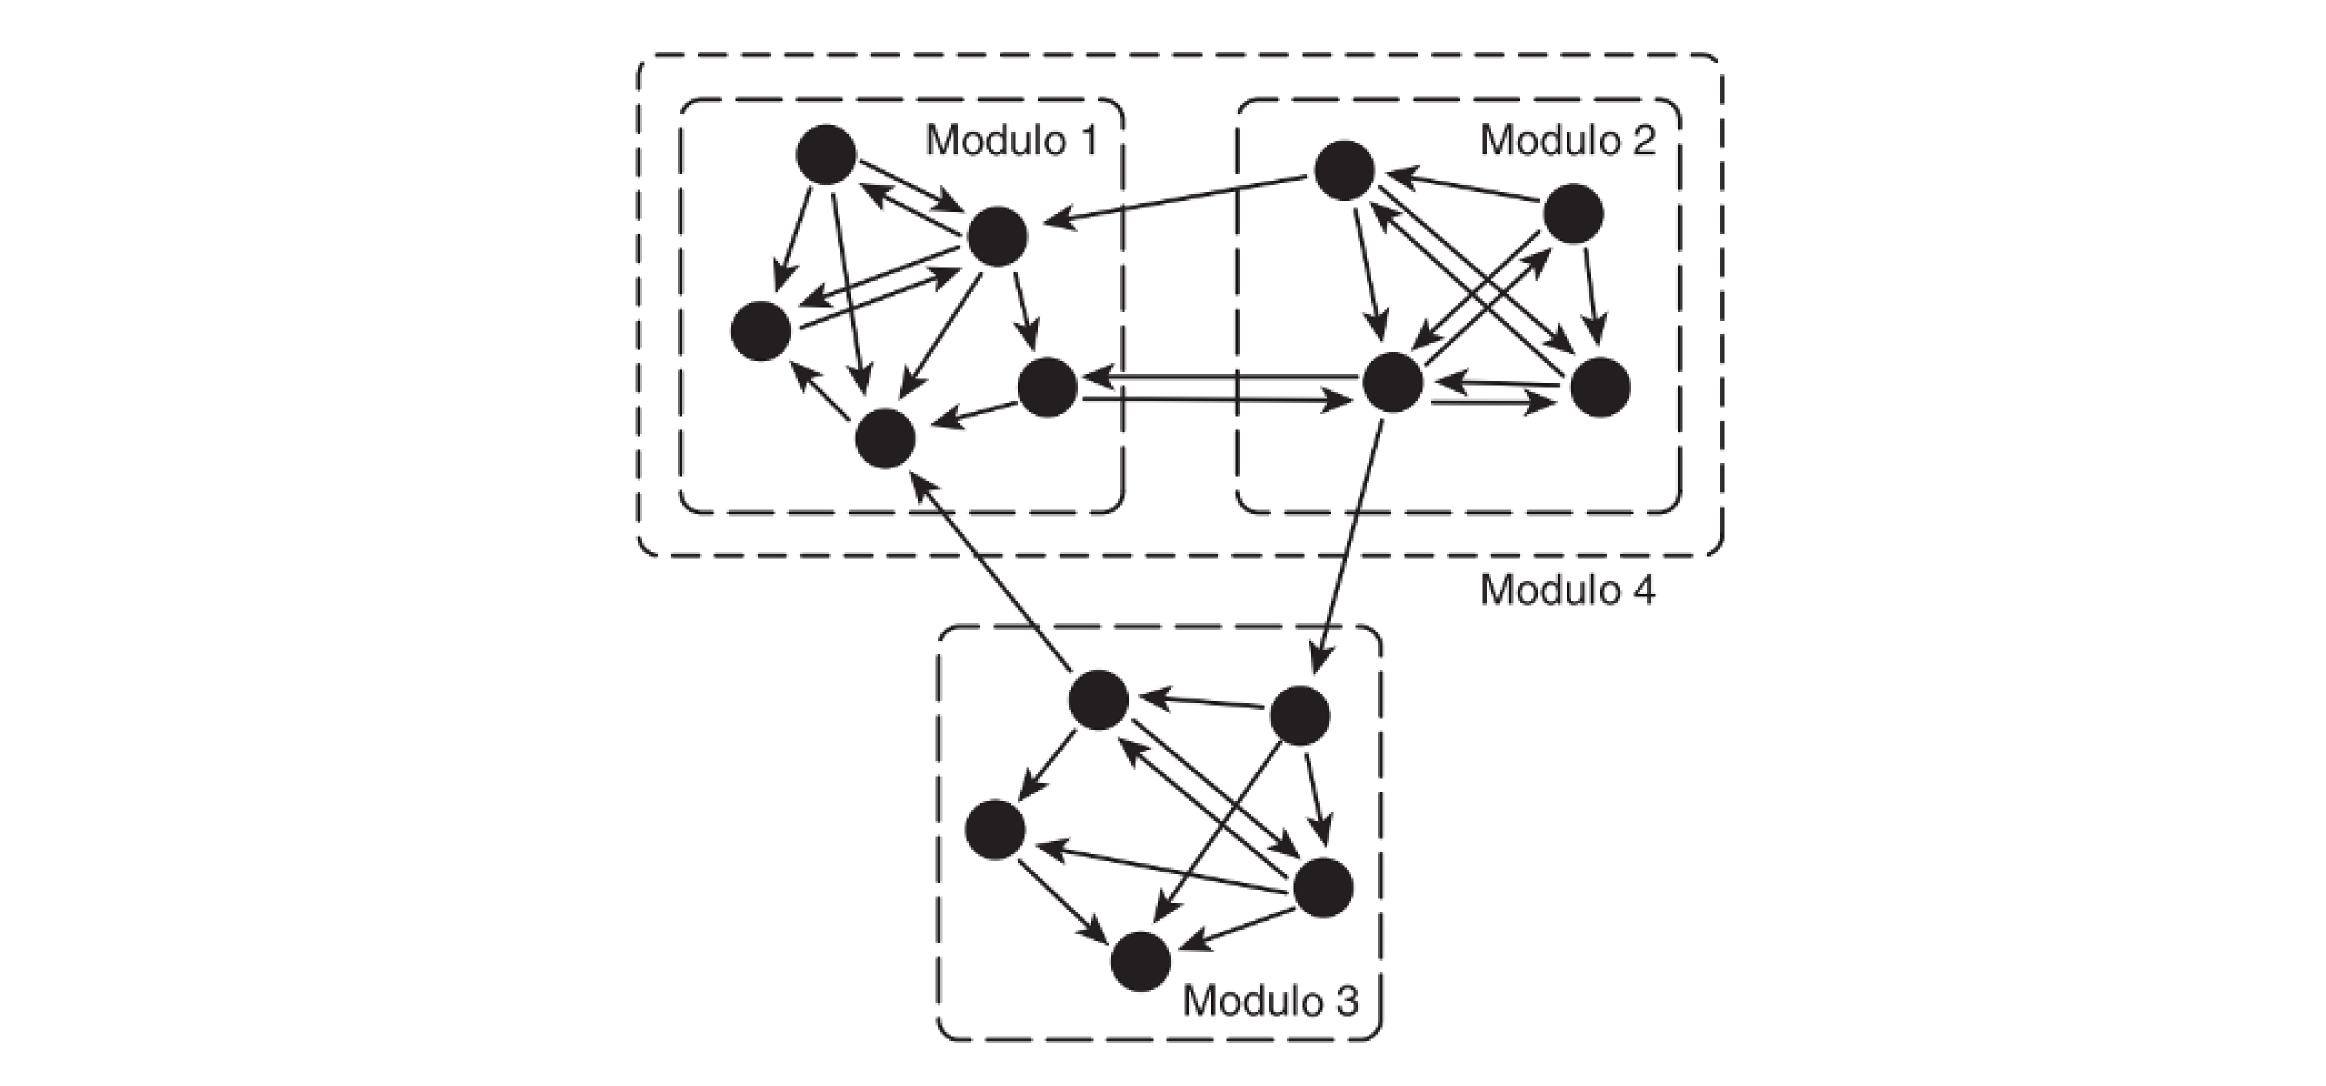
\includegraphics{./figuras/modulos.png}
\caption{Representação esquemática da organização modular dos seres
vivos. As setas representam qualquer tipo de relação entre as partes de
um indivíduo. Adaptado de Klingenberg 2008.}
\label{modulos}
\end{marginfigure}

Podemos classificar os tipos de módulos de acordo com o tipo de
interação que os define \cite{Wagner2007}. Porém, todos os níveis de
modularidade estão relacionados, e não podemos tratar de um sem
considerar o outro.

\begin{description}
\item[Módulo funcional:]
Alguns caracteres agem conjuntamente no desempenho de funções
biológicas. Pensando no crânio de mamíferos, os ossos da região da face
estão envolvidos em diversas funções, como mastigação, olfação ou visão.
No caso da mastigação, por exemplo, se espera que as mandíbulas
inferiores e superiores trabalhem de forma conjunta no desempenho dessa
função, e isso impõem restrições na forma e tamanho dos ossos envolvidos
nessa tarefa. Já os ossos que compõem o neurocrânio estão relacionados
com a proteção do cérebro dos mamíferos, e não tem relação direta com a
mastigação. Essa separação em regiões funcionais diferentes tem
consequências para o organismo.
\item[Módulo de desenvolvimento:]
Durante o desenvolvimento, caracteres podem se comportar de forma quase
autônoma dentro de um embrião com relação aos seus processos de
crescimento e diferenciação. Ou ainda, genes e proteínas podem estar
envolvidos em uma cascata autônoma de sinalização que faz parte do
desenvolvimento do organismo. Voltando ao exemplo acima dos dois módulos
funcionais nos mamíferos, estes mesmos módulos possuem origem
embrionária distinta. O desenvolvimento da face dos mamíferos provém do
crescimento e da diferenciação de células da mesoderme paraxial,
enquanto que o desenvolvimento do neurocrânio se dá a partir das células
da crista neural. Esses dois tecidos embrionários não influenciam o
desenvolvimento um do outro, portanto são partes praticamente autônomas
do embrião. Assim, os dois módulos funcionais, face e neurocrânio dos
mamíferos, também são dois módulos de desenvolvimento distintos.
\item[Módulo variacional:]
Os módulos variacionais são caracterizados por correlações altas entre
caracteres dentro do módulo e correlações baixas entre caracteres de
módulos diferentes. Enquanto as definições de módulos funcionais e de
desenvolvimento referem-se a fenômenos do indivíduo, o módulo
variacional é um fenômeno populacional. Apesar dos caracteres
pertencerem a organismos individuais, suas correlações só podem ser
determinadas em um estudo populacional. As correlações encontradas
refletem organizações modulares tanto no desenvolvimento quanto na
estrutura genética dos indivíduos, e são moldadas por demandas
evolutivas \cite{Klingenberg2008}.
\end{description}

\section{Integração Morfológica}\label{integrauxe7uxe3o-morfoluxf3gica}

No contexto de caracteres contínuos, a teoria da integração morfológica
foi inicialmente elaborada por Olson e Miller em seu livro ``Integração
Morfológica''. Neste livro, os autores apresentam a integração
morfológica como uma forma de estudar a evolução dos animais como
organismos totais, concebendo-os como uma abstração, baseada em
associações entre medidas \cite{Olson1958}. Estas associações de
medidas são representadas por correlações fenotípicas e organizadas em
módulos variacionais. A relevância em se investigar complexos de
caracteres em vez de caracteres isolados está na visão de que mudanças
em um caráter podem não ser independentes de mudanças em outros
caracteres do organismo. Olson e Miller já ponderavam sobre as relações
entre magnitude de integração e evolução. Seria a intensidade de
integração, ou seja, o quão fortemente os caracteres estão associados
entre si, capaz de influenciar a evolução de organismos mais complexos e
seu grau de adaptabilidade? Pensando em magnitudes de integração, esses
autores compreenderam a importância da dualidade integração-modularidade
no potencial de evolução morfológica, ou seja, que esses dois conceitos
são os dois lados de uma mesma moeda. Modularidade permite com que
caracteres se comportem de forma independente, enquanto integração
garante que mudanças em um caráter sejam coordenadas com mudanças nos
demais caracteres que interagem com o primeiro. Na próxima seção vamos
discutir essa dualidade em detalhes num contexto evolutivo.

Günter P. Wagner \cite{Wagner1996} ressaltou que é preciso haver uma
razão biológica para que o plano corpóreo dos organismos seja organizado
de maneira tão obviamente modular, tornando facilmente reconhecíveis
suas unidades naturais (como mostrado pela nossa capacidade de apontar
estruturas homólogas). Para ele, considerar as unidades naturais como
unidades de transformação evolutiva (ou seja, a modularidade como uma
propriedade variacional do genoma) traz o sentido biológico dessa
organização. Segundo ele, três critérios precisam ser satisfeitos para
um complexo de caracteres ser considerado como uma unidade modular: (1)
servir a uma função primária; (2) ser integrado por efeitos
pleiotrópicos; e (3) ser relativamente independente de outras unidades.
A visão de Wagner leva a uma estrutura particular do mapa
genótipo-fenótipo dentro de um individuo, no qual genes estariam
divididos em grupos com efeitos pleiotrópicos localizados, restritos a
caracteres envolvidos com uma determinada função. Essa organização
modular do mapa genótipo-fenótipo seria responsável ela organização dos
caracteres em módulos variacionais.

\begin{figure}
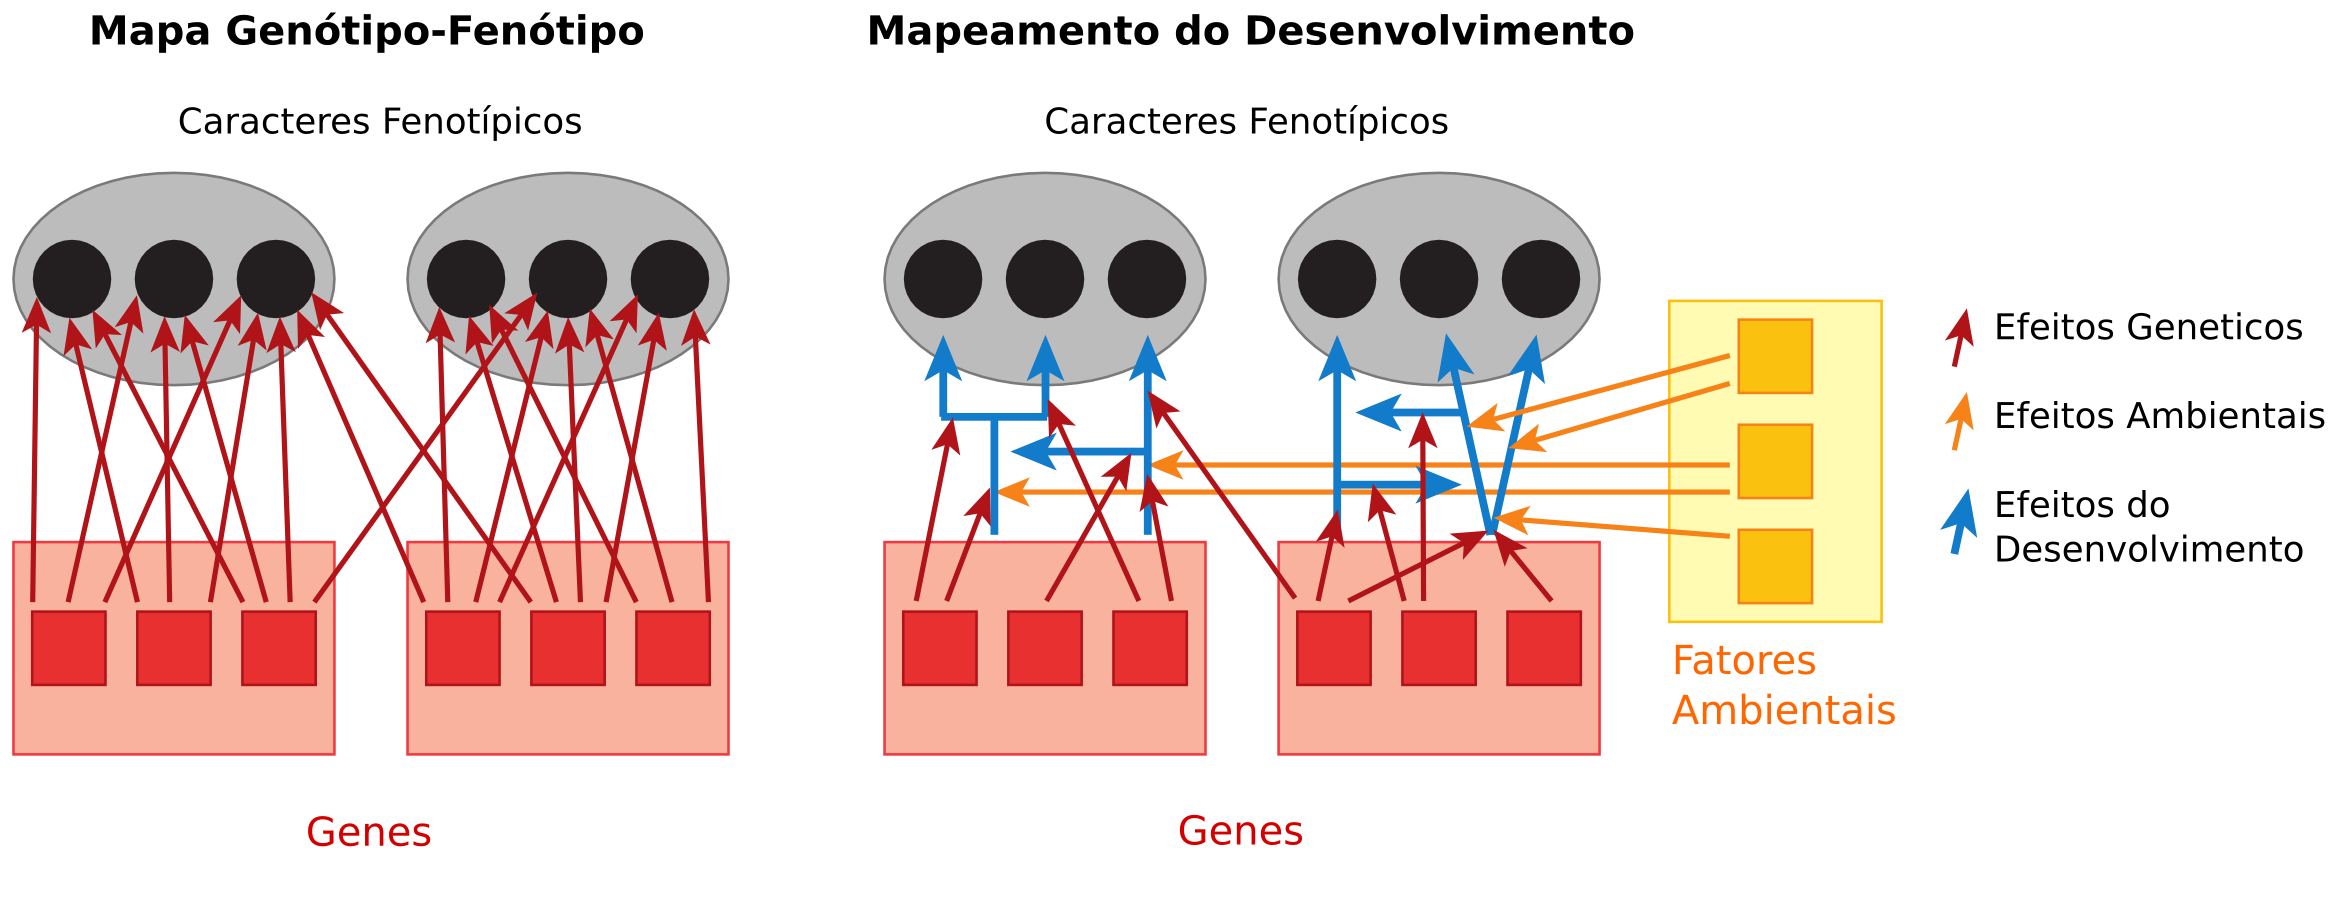
\includegraphics{./figuras/mapgenfen.png}
\caption{Mapa genótipo-fenótipo modular clássico, e mapa incluindo
efeitos do desenvolvimento. Adaptado de Klingenberg 2008.}
\label{mapagenfen}
\end{figure}

\section{Consequências Evolutivas}\label{consequuxeancias-evolutivas}

A organização modular do genoma e do desenvolvimento e a consequente
estrutura variacional modular leva a consequências evolutivas
importantes. Quando grupos de caracteres constituem um módulo e
provavelmente funcionam de forma integrada no desempenho de um função,
seleção sobre um dos caracteres, produzindo mudanças em uma parte do
módulo, poderia ocasionar uma disrupção na composição harmoniosa desse
conjunto de características. Porém, a alta correlação entre caracteres
de um módulo impede que isso aconteça, pois respostas correlacionadas
são observadas nos caracteres que não estão sobre seleção, e todos os
caracteres do módulo acabam por se modificarem de forma conjunta,
mantendo sua harmonia interna. De forma complementar, se todos os
caracteres do organismo fossem integrados, seleção em um caráter
provocaria mudanças em todos os outros, até aqueles relacionados com
outras funções ou em partes distantes do organismo. A divisão em módulos
permite que partes diferentes se modifiquem de forma relativamente
independente. Evolutivamente, então, integração e modularidade permitem
que grupos de características funcionalmente ou ontogeneticamente
ligadas se modifiquem de forma harmoniosa; e que características em
módulos diferentes possam se alterar de forma relativamente
independente.

\section{Autovalores e Autovetores}\label{autovalores-e-autovetores}

Quando trabalhamos com muito caracteres, avaliar ao mesmo tempo a
evolução e a variação de todos simultaneamente se torna pouco factível.
Para sanar essa dificuldade, podemos nos valer de alguns tipos de
transformação das variáveis que tragam simplificações ou características
marcantes das populações estudadas. Uma forma de transformação é a
analise de componentes principais, também conhecida como decomposição de
autovalores e autovetores.

Os autovetores, ou componentes principais, nada mais são que as direções
de maior variação não correlacionadas (Fig. \ref{autovetores}).

\begin{marginfigure}
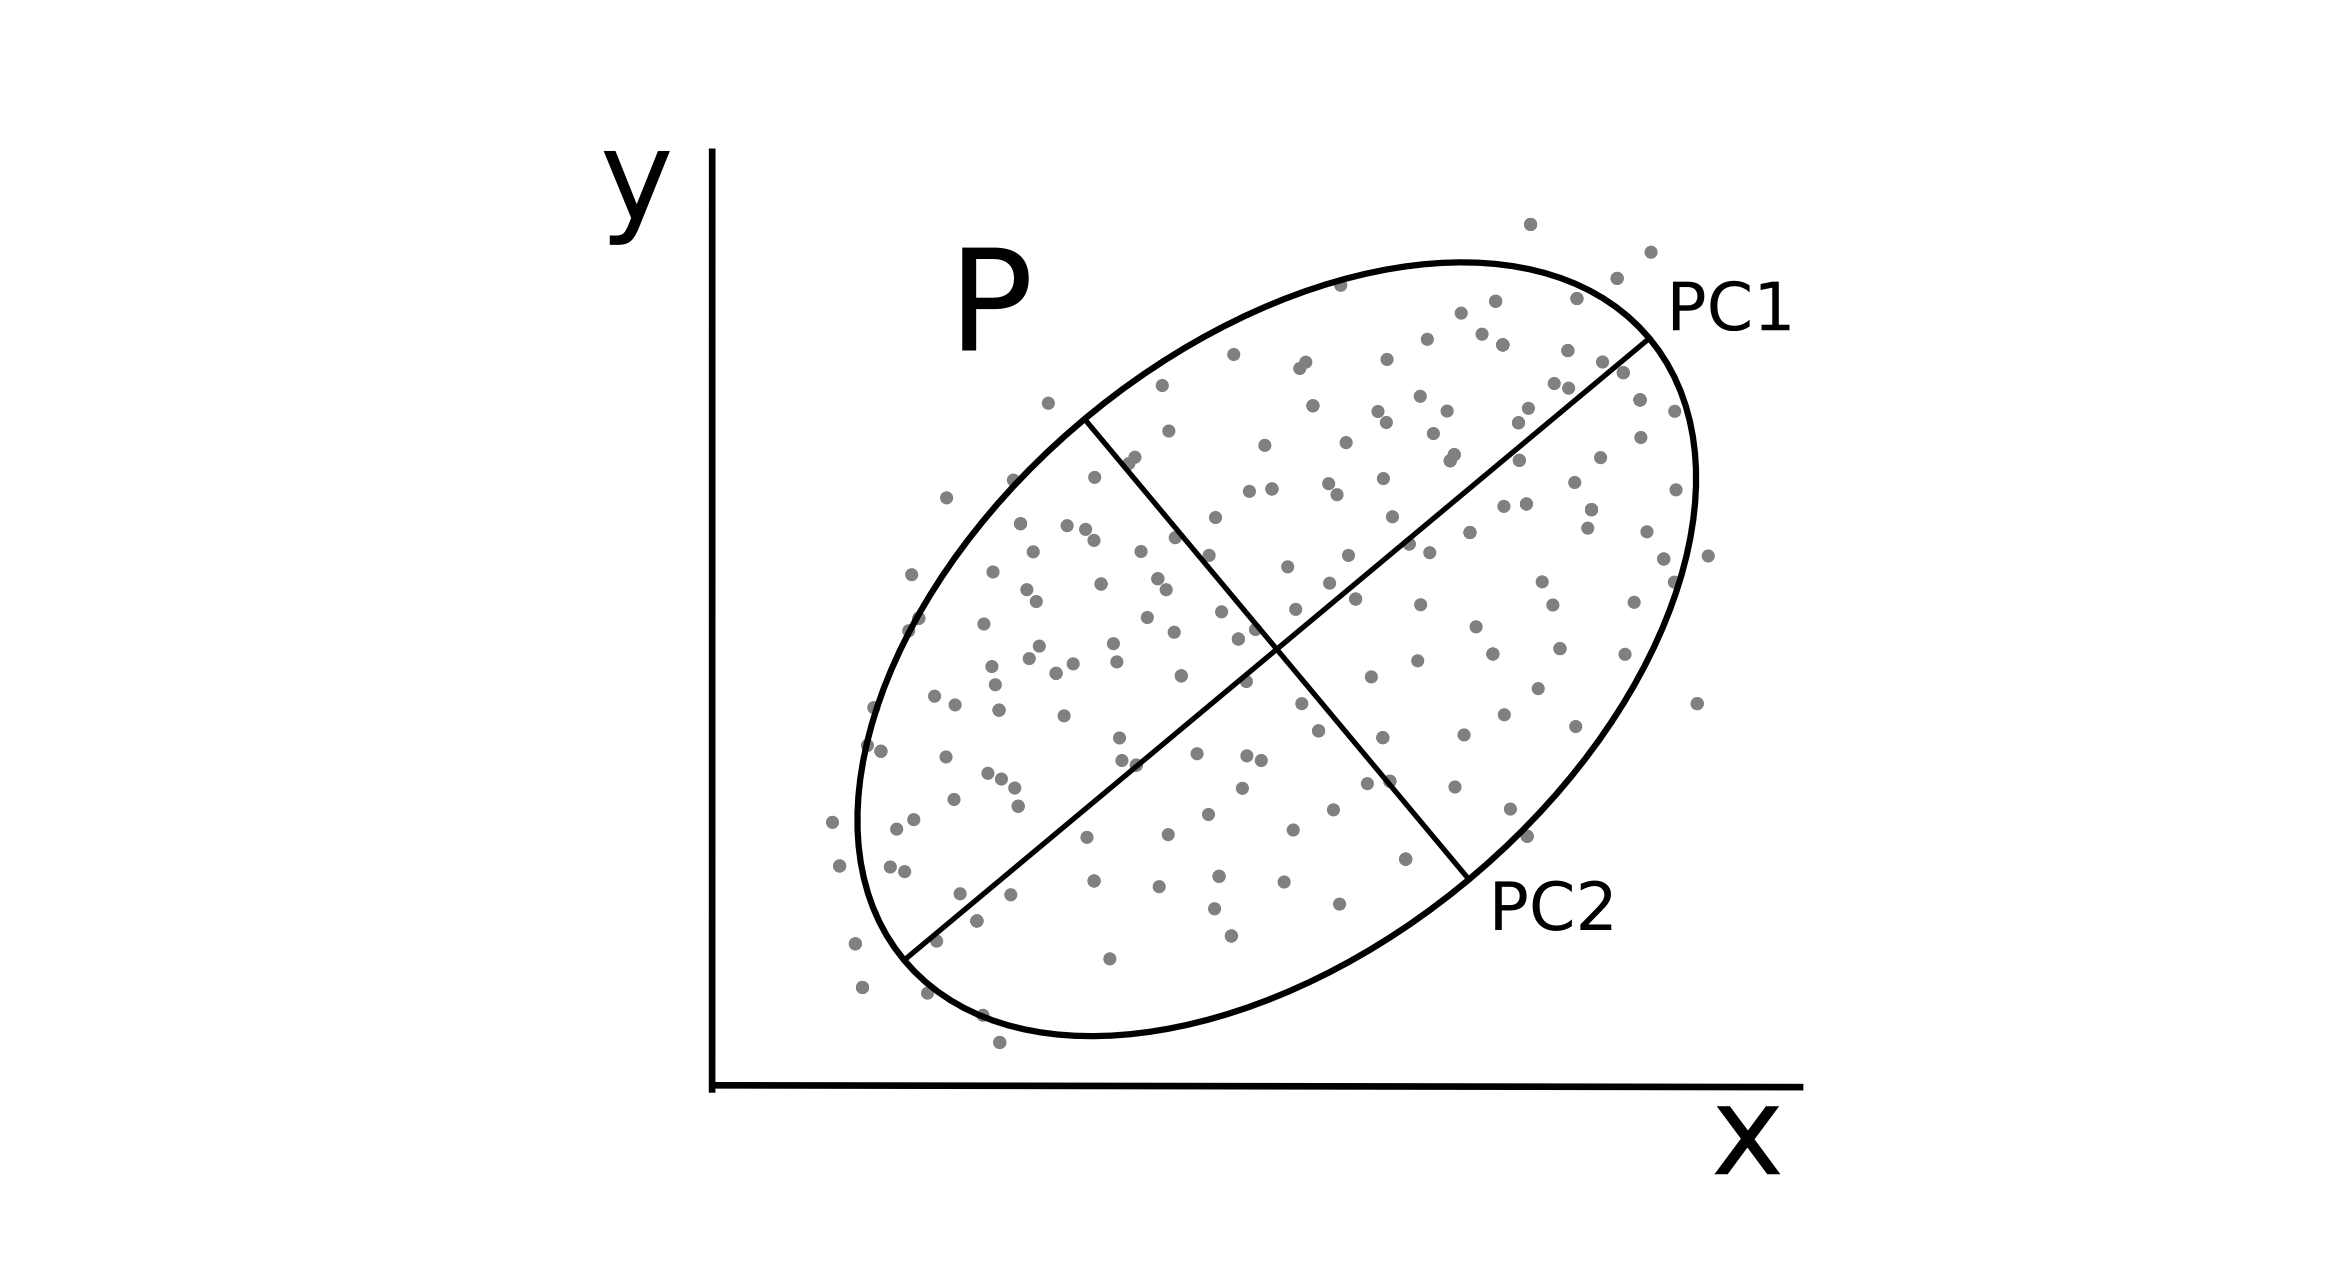
\includegraphics{./figuras/auto-vetores.png}
\caption{Autovetores da distribuição dos caracteres X e Y. PC1
representa o primeiro componente principal da matriz \(\mathbf{P}\), ou
primeiro autovetor, e corresponde ao eixo de maior variação fenotípica.
PC2, então, representa o segundo eixo de maior variação ortogonal ao
primeiro.}
\label{autovetores}
\end{marginfigure}

A quantidade de variação em cada direção dos componentes principais é
medida pelo seu autovalor correspondente. O primeiro autovetor é
associado ao maior autovalor. O autovalor nada mais é que a variância na
direção do autovetor correspondente.

O numero de autovetores e autovalores é dado pela dimensão do espaço que
estamos trabalhando, ou seja, o número de caracteres estudados. Para
cada \(p\) caracteres, teremos \(p\) autovetores. Porém, na maior parte
dos sistemas morfológicos, grande parte da variação está concentrada nos
primeiros componentes principais, e portanto podemos caracterizar de
forma bastante completa a variação na população utilizando estes
primeiros componentes.

\section{Tamanho e Linhas de Menor Resistência
Evolutiva}\label{tamanho-e-linhas-de-menor-resistuxeancia-evolutiva}

Os componentes principais trazem uma informação importante sobre a
distribuição de variação no morfoespaço. Lembrando que a seleção natural
sempre atua sobre variação existente na população, podemos pensar no
primeiro componente principal, o eixo de maior variação, como uma
direção especialmente favorável para a resposta à seleção. Por esse
motivo, essa direção ficou conhecida como linha de menor resistência
evolutiva \cite{Schluter1996}. Frequentemente, vemos a linha de
menor resistência evolutiva enviesando o vetor de resposta à seleção,
mesmo quando o gradiente de seleção está orientado em outra direção
\cite{Marroig2005}. Esse desvio se dá pela ação da seleção indireta,
descrita nas seções anteriores (fig. \ref{desvio-trajetorias}). Quando
maior for a porção da variação presente no primeiro componente
principal, maior será o desvio da seleção em direção à linha de menor
resistência evolutiva.

Na maior parte dos mamíferos, podemos identificar o primeiro componente
principal com uma característica bastante simples: Tamanho. Essa
identificação vem do fato de todos os componentes do primeiro autovetor
terem, frequentemente, o mesmo sinal. Mudanças evolutivas ao longo desse
eixo do morfoespaço representam, portanto, alteração coordenadas entre
todos os caracteres avaliados, ou seja, todos aumentam ou diminuem
juntos. Assim, essas mudanças representam mudanças de tamanho, e o
principal eixo de variação dentro de populações é no tamanho dos
indivíduos \cite{Porto2009}.

\bibliography{apostila}
\bibliographystyle{abbrv}

\end{document}
